%% LyX 2.2.2 created this file.  For more info, see http://www.lyx.org/.
%% Do not edit unless you really know what you are doing.
\documentclass[a4paper,english,twoside]{memoir}
\usepackage{lmodern}
\usepackage[LGR,T1]{fontenc}
\usepackage[latin9]{inputenc}
\setcounter{secnumdepth}{3}
\setcounter{tocdepth}{3}
\usepackage{color}
\usepackage{babel}
\usepackage{units}
\usepackage{textcomp}
\usepackage{amstext}
\usepackage{graphicx}
\usepackage[unicode=true,
 bookmarks=true,bookmarksnumbered=false,bookmarksopen=false,
 breaklinks=false,pdfborder={0 0 0},pdfborderstyle={},backref=false,colorlinks=true]
 {hyperref}
\hypersetup{pdftitle={simetuc User Manual},
 pdfauthor={Pedro Villanueva-Delgado}}

\makeatletter

%%%%%%%%%%%%%%%%%%%%%%%%%%%%%% LyX specific LaTeX commands.
\pdfpageheight\paperheight
\pdfpagewidth\paperwidth

\DeclareRobustCommand{\greektext}{%
  \fontencoding{LGR}\selectfont\def\encodingdefault{LGR}}
\DeclareRobustCommand{\textgreek}[1]{\leavevmode{\greektext #1}}
\ProvideTextCommand{\~}{LGR}[1]{\char126#1}


%%%%%%%%%%%%%%%%%%%%%%%%%%%%%% User specified LaTeX commands.
\usepackage[dvipsnames]{xcolor}

\@ifundefined{showcaptionsetup}{}{%
 \PassOptionsToPackage{caption=false}{subfig}}
\usepackage{subfig}
\makeatother

\usepackage{listings}
\lstset{basicstyle={\ttfamily},
backgroundcolor={\color{black!10}},
framexleftmargin=0em,
columns=flexible}
\renewcommand{\lstlistingname}{Listing}

\begin{document}

\title{\emph{simetuc} User Manual}

\author{Pedro Villanueva-Delgado}

\maketitle
\tableofcontents{}

\chapter{Features}
\begin{itemize}
\item Command line interface program.

\begin{itemize}
\item Run with 
\begin{lstlisting}[basicstyle={\ttfamily}]
simetuc config_file.txt [options]
\end{lstlisting}
\item See help and all options with 
\begin{lstlisting}
simetuc -h
\end{lstlisting}
\end{itemize}
\item The simulation is controlled by a configuration text file that the
user can edit with the parameters adequate to the system of study.
It includes:

\begin{itemize}
\item Information about the host lattice.
\item Energy states labels.
\item Absorption and excitation (including ESA).
\item Decay (including branching ratios).
\item Energy transfer.
\item Other settings for the power and concentration dependence or optimization. 
\end{itemize}
\item \emph{simetuc} works with any sensitizer and activator ion kind.

\begin{itemize}
\item The examples are given for the Yb-Tm system. 
\end{itemize}
\item All kinds of energy transfer processes are supported:

\begin{itemize}
\item Energy migration.
\item Upconversion (ETU).
\item Downconversion.
\item Cross-relaxation.
\item Cooperative processes.
\item Energy transfer from sensitizers to activators.
\item Back transfer from activators to sensitizers. 
\end{itemize}
\item See the example configuration file in the simetuc folder.

\begin{itemize}
\item The configuration file sections are detailed and discussed in this
document.
\item See also the full example in the appendix.
\end{itemize}
\item Add decay experimental data as two column text data, separated by
tabs or spaces.
\item Different options:

\begin{itemize}
\item Create the lattice.
\item Simulate the dynamics (rise and decay).
\item Optimize the energy transfer parameters. 

\begin{itemize}
\item Minimize the deviation between experiment and simulation.
\end{itemize}
\item Simulate the steady state.
\item Simulate the power dependence of each emission.
\item Simulate the concentration dependence of the dynamics or the steady
state.
\end{itemize}
\item All results are plotted and saved in the .hdf5 format.
\item For all options \lstinline!--average! uses standard average rate
equations instead of microscopic ones.
\end{itemize}

\chapter{Installation}

Python 3.5 or 3.6 is required. Installing Anaconda is recommended;
it works with Windows (64/32 bits), Linux (64/32 bits) and Mac (64
bits).

After installing \href{https://www.continuum.io/downloads}{Anaconda},
execute the following commands at the command prompt (\emph{cmd.exe}
for Windows, \emph{shell} for Linux and Mac):\footnote{Some OSX users report problems using \emph{conda}, if after installing
you can't use the program (i.e., \emph{simetuc -h} fails because \emph{simetuc}
wasn't recognized as a command), use \emph{pip install simetuc.}}

\begin{lstlisting}
conda config --add channels conda-forge
conda config --add channels pedvide
conda install simetuc
\end{lstlisting}

(The first two commands add package repositories with up-to-date versions
of all needed packages.)

or

\begin{lstlisting}
pip install simetuc
\end{lstlisting}

That will download and install all necessary files.

Check that the program was installed correctly with

\begin{lstlisting}
simetuc -h
\end{lstlisting}

which should display something similar to Figure \ref{fig:simetuc-h}.

\begin{figure}
\begin{centering}
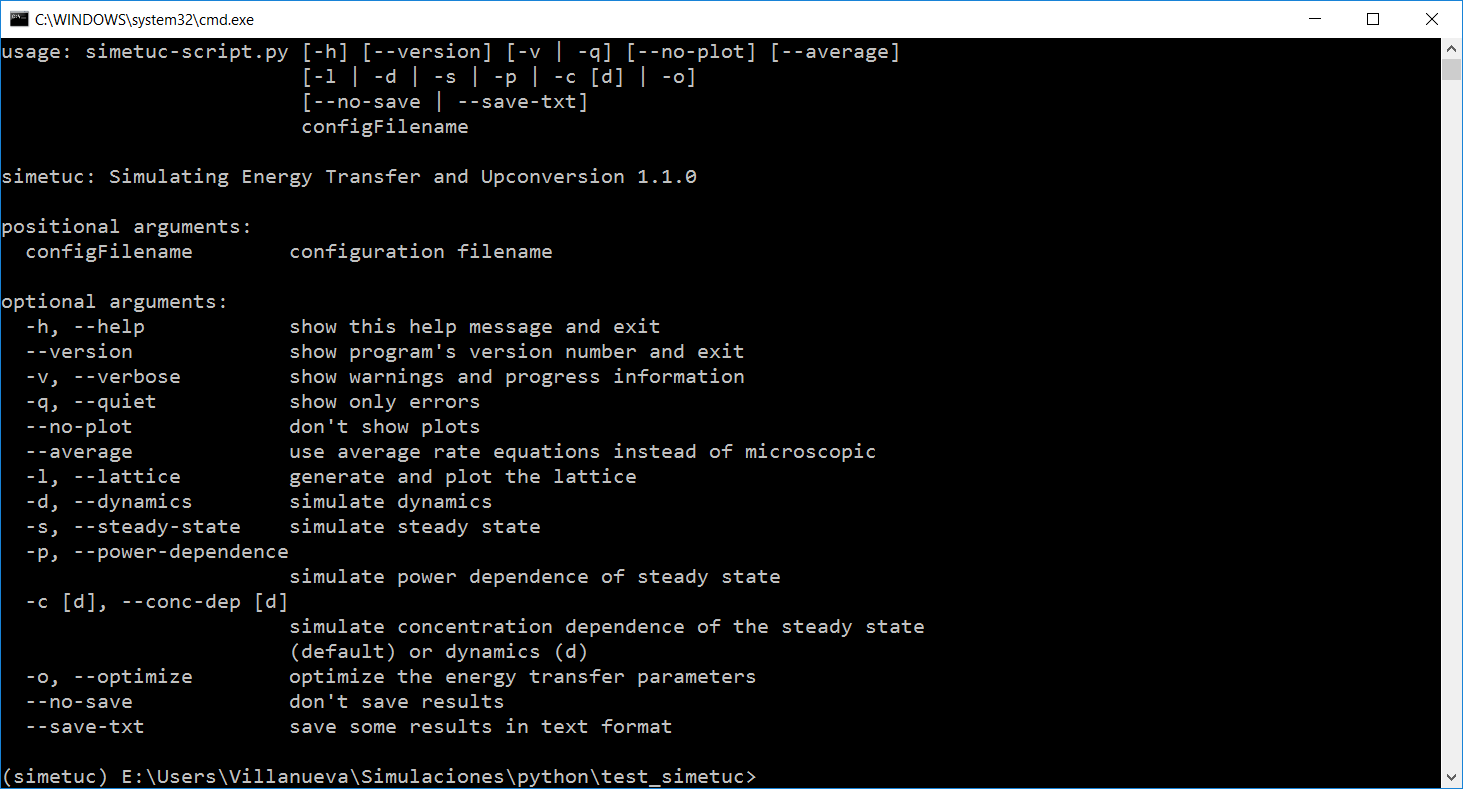
\includegraphics[width=1.2\textwidth]{figures/simetuc_help.PNG}
\par\end{centering}
\caption{\label{fig:simetuc-h}Results of \texttt{simetuc -h}.}

\end{figure}


\section{Update}

If you installed it using \emph{conda}, update with:

\begin{lstlisting}
conda update -c pedvide simetuc
\end{lstlisting}

If you installed it with \emph{pip}, update with:

\begin{lstlisting}
pip install -U simetuc 
\end{lstlisting}


\chapter{The configuration file}

Some sections of the configuration file are mandatory (the starred
Sections \ref{subsec:Version}-\ref{subsec:Decay}), some are optional
(Sections \ref{subsec:Branching-ratios}-\ref{subsec:Optimization-Method}),
and some are only mandatory when performing a particular simulation
type (Sections \ref{subsec:Power-Dependence} and \ref{subsec:Concentration-Dependence}).

Comments can be placed anywhere in the file starting with a hash symbol
(\#).

The different sections of the file begin by a section name, for example
lattice or states, followed by a colon (:). The different subsections
and values are in a new line and indented with four spaces (not tabs!).
A section can contain a single value or subsections; for example:

\begin{lstlisting}
# comment1
section1: value1
section2:
    subsection1: value2 # comment2
    subsection2:
        subsubsection1: value3
\end{lstlisting}

Some of the values may be text or numbers, others, however, may be
lists or a list of lists. A list is written as a comma-separated values
between two square brackets:

\begin{lstlisting}
section: [item1, item2, item3]
\end{lstlisting}

And for a list of lists:

\begin{lstlisting}
section: [[lst1_item1, lst1_item2], [lst2_item1, lst2_item2]]
\end{lstlisting}

A full example of a configuration file, showing all options, is shown
in Listing \ref{lst:full_conf_file}.

\section{\label{subsec:Version}Version{*}}

At the moment, there is only one format for the configuration file;
however, in the future, it is possible that an improved format is
introduced that is not compatible with the current one. For this reason
the version of the format has to be included, the only value allowed
is 1:

\begin{lstlisting}
version: 1
\end{lstlisting}


\section{Lattice{*}\label{subsec:Lattice}}

This section defines the name of the lattice, the unit cell parameters,
the concentration of sensitizer and activator ions, and optionally,
a maximum distance of interaction.

This section starts with
\begin{lstlisting}
lattice:
    # values and subsections...
\end{lstlisting}

Those values and subsections are described now.
\begin{description}
\item [{The~name}] is an arbitrary text that describes the lattice. It
will be used as a folder name under latticeData (Section \ref{subsec:The-latticeData-folder}),
expData (Section \ref{subsec:The-expData-folder}), and results (Section
\ref{sec:The-results-folder}). Therefore it should only contain letters,
numbers, and underscore (\_) characters (no spaces).
\item [{The~number~of~unit~cells}] is an integer greater than zero.
It specifies how many unit cells along the three directions a lattice
will consist of. 
\item [{The~concentration}] of sensitizer and activator, in percentages
from 0 to 100\%. An ion with 0\% concentration will not participate
in the equations and therefore will not make the simulation take longer.
\begin{lstlisting}
    S_conc: 0
    A_conc: 0.3
\end{lstlisting}
\item [{The~unit~cell~parameters}] consist of the three lattice distances
and three angles. The distances are given in Angstrom and the angles
in degrees (between 0 and 360�). 
\begin{lstlisting}
    # distances in Angstrom
    a: 5.9738
    b: 5.9738
    c: 3.5297
    # angles in degree
    alpha: 90
    beta: 90
    gamma: 120
\end{lstlisting}
\item [{The~spacegroup}] determines the symmetry of the lattice. It can
be given as the international short symbol (e.g., P-6) or as the International
Union of Crystallography number (e.g. 174). 
\item [{The~sites}] positions and occupancies determine the positions
of the doped ions (in units of the lattice distances, from 0 to 1)
and their fractional occupancy (between 0 and 1). For a lattice with
just one site: 
\begin{lstlisting}
    sites_pos: [0, 0, 0]
    sites_occ: 1
\end{lstlisting}
For a lattice with two sites, the second of which is half occupied:
\begin{lstlisting}
    sites_pos: [[0, 0, 0], [2/3, 1/3, 1/2]]
    sites_occ: [1, 1/2]
\end{lstlisting}
The sites are populated randomly using the desired concentration,
see Section \ref{sec:Creating-a-lattice}.
\end{description}
A full example of the lattice section is

\begin{lstlisting}
lattice: # all fields here are mandatory
    name: bNaYF4
    N_uc: 40
    S_conc: 0
    A_conc: 0.3
    # unit cell
    # distances in Angstrom
    a: 5.9738
    b: 5.9738
    c: 3.5297
    # angles in degree
    alpha: 90
    beta: 90
    gamma: 120
    spacegroup: P-6
    # info about sites.
    sites_pos: [[0, 0, 0], [2/3, 1/3, 1/2]]
    sites_occ: [1, 1/2]
\end{lstlisting}


\subsection{Optional values}
\begin{description}
\item [{The~maximum~distances}] for the normal and cooperative interactions
restrict energy transfer to ions closer than the distances. The normal
maximum distance (\texttt{d\_max}) is not yet implemented; however,
the cooperative one is, and it's strongly recommended to use it if
cooperative interactions are present. The cooperative interactions
grow approximately with the cube of the number of ions, the normal
interactions grow with the square.\\
If the values are not present, they are set to infinite.
\begin{lstlisting}
lattice:
    ... all other fields ... 
    d_max: 100.0
    d_max_coop: 25.0
\end{lstlisting}
\end{description}

\section{States{*}\label{subsec:States}}

This section determines the number of energy states per ion and their
labels.

Four subsections are mandatory, two per ion type:
\begin{description}
\item [{The~ion~labels}] is any text that describes the sensitizer or
activator ion. It usually is the ion's chemical symbol.
\item [{The~ion~states~labels}] is a list of text. Each item in the
list labels an energy state; the first is the ground state, the rest
should be in order of increasing energy. Usually the term symbols
of the Dieke diagram are used.
\end{description}
\begin{lstlisting}
states:
    sensitizer_ion_label: Yb
    sensitizer_states_labels: [GS, ES]
    activator_ion_label: Tm
    activator_states_labels: [3H6, 3F4, 3H5, 3H4, 3F3, 1G4, 1D2]
\end{lstlisting}

The ion and state labels will be used to define excitation (Section
\ref{subsec:Excitation}), decay (Section \ref{subsec:Decay}), branching
ratios (Section \ref{subsec:Branching-ratios}), and energy transfer
processes (Section \ref{subsec:Energy-Transfer}).

\section{Excitation{*}\label{subsec:Excitation}}

At the beginning of the simulation, all ions are in their ground state.
An excitation source is necessary to pump them to an excited state.
This source can be pulsed for dynamics or continuous for steady state
simulations.

Any number of excitation subsections can be added to the file, and
at least one has to be active (see below). A two-color experiment
can be simulated by activating two excitations. Any number of excitations
can be active.

An excitation block contains several mandatory subsections:
\begin{description}
\item [{The~label}] is a short unique text. It identifies the excitation
and it is used in the naming of experimental data files (see Section
\ref{subsec:The-expData-folder}), so short, informative names are
encouraged. 
\item [{active}] can be true or false and indicates whether the excitation
will be used for the simulations. 
\item [{The~excitation~power~density}] in $\unit{W\,cm^{-2}}$. For
pulsed sources this has to be the instantaneous power density of the
pulse. Usual values are in the order of $\unit[10^{5}\text{\ensuremath{-}}10^{7}]{W\,cm^{-2}}$
for pulsed excitations and $\unit[10^{1}\text{\ensuremath{-}}10^{3}]{W\,cm^{-2}}$
for continuous excitations. 
\item [{The~pulse~width}] of the excitation source (in seconds) for pulsed
excitations. For continuous excitations it can be omitted. 
\item [{The~process}] is the actual absorption transition. The format
is \texttt{ion\_label(state\_label\_i) -> ion\_label(state\_label\_f)}.
Where the ion and state labels were defined in Section \ref{subsec:States}.
Both ion labels have to be present and equal; both state labels have
to belong to the same ion type. 
\item [{The~degeneracy}] is the relative degeneracy of the initial and
final states. The relative degeneracy of two trivalent lanthanide
states with terms $^{2S_{i}+1}L_{iJ_{i}}$ and $^{2S_{f}+1}L_{fJ_{f}}$
is $g_{rel}=\frac{2J_{i}+1}{2J_{f}+1}$. 
\item [{The~pump~rate}] is the absorption cross-section divided by the
transition energy in units of $\unit{cm^{2}\,J^{-1}}$, that is $R_{P}=\frac{\sigma(\nu)}{h\nu}$.
The pump rate multiplied by the power density is equal to the absorption
probability, with units of $\unit{s^{-1}}$. 
\end{description}
An example with two excitation blocks:

\begin{lstlisting}
excitations:
    pulsed_1G4:
        active: True
        power_dens: 1e6
        t_pulse: 1e-8
        process: Tm(3H6) -> Tm(1G4)
        degeneracy: 13/9
        pump_rate: 9.3e-4
    CW_980nm:
        active: False
        power_dens: 1e2
        process: Yb(GS) -> Yb(ES)
        degeneracy: 4/3
        pump_rate: 4.4e-3
\end{lstlisting}


\subsection{Excited state absorption}

Excited state absorption (ESA) can be simulated by giving a list of
transitions, degeneracies and pump rates in the corresponding fields,
for example:

\begin{lstlisting}
excitations:
    NIR_800:
        active: False
        power_dens: 1e5
        t_pulse: 1e-8
        process: [Tm(3H6)->Tm(3H4), Tm(3H5)->Tm(1G4)] # list
        degeneracy: [13/9, 11/9] # list
        pump_rate: [4.4e-3, 4e-3] # list
\end{lstlisting}


\section{\label{subsec:Decay}Decay{*}}

This section contains the decay lifetimes in seconds. There are two
sections, one for the sensitizer and one for the activator. In both
cases the decay lifetimes are input with \texttt{state\_label: lifetime}:

\begin{lstlisting}
sensitizer_decay:
    ES: 2.5e-3
activator_decay:
    3F4: 12e-3
    3H5: 25e-6
    3H4: 2e-3
    3F3: 2e-6
    1G4: 760e-6
    1D2: 67.5e-6
\end{lstlisting}


\section{\label{subsec:Branching-ratios}Branching ratios}

These are two optional sections, one for the sensitizer and one for
the activator.

The branching ratios describe the fraction of emission from an initial
state to a final state. The format is \texttt{initial\_state -> final\_state: ratio.}
The ratio is a number between zero and one. The branching ratio to
the ground state does not need to be specified because it is calculated
automatically from the other values.

\begin{lstlisting}
sensitizer_branching_ratios: # can be empty or simply omitted
activator_branching_ratios:
    3H5->3F4: 0.4
    3H4->3F4: 0.3
    3H4->3H5: 0.1
    3F3->3H4: 0.999
    1G4->3F4: 0.15
    1G4->3H5: 0.16
    1G4->3H4: 0.04
    1G4->3F3: 0.001
    1D2->3F4: 0.43
\end{lstlisting}


\subsection{Multiphonon relaxation and thermalization}

When two states are close in energy, the upper one can decay nonradiatively
to the lower one in a process known as multiphonon relaxation. This
process can be described in the configuration file as a branching
ratio from the upper to the lower state with the appropriate value.
In the example above, the $^{3}$F$_{3}$ state decays into the $^{3}$H$_{4}$
state with a branching ratio of 0.999; this means that the MPR rate
is $k_{MPR}=0.999\cdot k_{^{3}\hspace{-2bp}F_{3}}$, where $k_{^{3}\hspace{-2bp}F_{3}}$
is the total decay rate given in section \ref{subsec:Decay}. The
radiative decay rate to the ground state is then $k_{rad}=(1-0.999)\cdot k_{^{3}\hspace{-2bp}F_{3}}$.

The lower state can also populate the upper one via phonons, and after
some time a thermal equilibrium can be established. The ratio of the
populations of the upper and lower states is then given by the Boltzmann
distribution. This process can be described in the configuration file
as a branching ratio from the lower to the upper state with the appropriate
value. For example, if there is a thermal equilibrium between the
$^{3}$F$_{3}$ and $^{3}$H$_{4}$ states we need to define two branching
ratios in the configuration file, one for relaxation and the other
for thermalization:

\begin{lstlisting}
activator_branching_ratios:
...
    3F3->3H4: 0.999 # multiphonon relaxation
    3H4->3F3: 5e-5 # multiphonon thermalization
...
\end{lstlisting}

The value for the multiphonon thermalization branching ratio should
be 
\[
k_{MPT}=k_{MPR}\exp\left(-\frac{\Delta E}{kT}\right)=0.999\exp(-10)\approx5\,10^{-5}
\]

where $\Delta E=\unit[2000]{cm^{-1}}$ is the energy difference between
the states and $\unit[kT_{r}=200]{cm^{-1}}$ is the room temperature
energy.

\section{\label{subsec:Energy-Transfer}Energy transfer}

This optional section includes one or more energy transfer processes
between ions in the simulation. Each energy transfer block refers
to one process and contains several fields:
\begin{description}
\item [{The~label}] is a short unique text. It can also be used to restrict
the optimization to certain processes (Section \ref{subsec:Optimization-Processes}). 
\item [{The~process}] describes the ET interaction with the format \texttt{ion\_label1(init\_state)
+ ion\_label2(init\_state) -> ion\_label1(end\_state) + ion\_label2(end\_state)}.
Where the ion and state labels were defined in Section \ref{subsec:States}.
\item [{The~multipolarity}] of the interaction is an integer number, usually
6, 8 or 10.
\item [{The~strength}] of the interaction given in units of $\unit{s^{-1}\,\AA^{n}}$,
where $n$ is the multipolarity. Optionally, an interaction strength
for the average rate equation system can be given; this value is several
orders of magnitude lower than the microscopic value, see Section
\ref{sec:Microscopic-or-average}. If it is not given and the average
rate equations are solved, the normal strength will be used.
\end{description}
For example:

\begin{lstlisting}
enery_transfer:
    CR50:
        process: Tm(1G4) + Tm(3H6) -> Tm(3H4) + Tm(3H5)
        multipolarity: 6
        strength: 4.3057e+09
        strength_avg: 8e+03 # optional, only for average system
    EM:
        process:  Yb(ES) + Yb(GS) -> Yb(GS) + Yb(ES)
        multipolarity: 6
        strength: 4.50220614e+10
\end{lstlisting}


\subsection{Cooperative energy transfer}

Cooperative energy transfer processes involve three ions. Two ions
cooperatively transfer (receive) energy to (from) a third ion. The
format is very similar to the normal energy transfer processes, the
only field that changes is \texttt{process}. It now must contain the
ion and state labels of three initial states and three final states,
for example:

\noindent %
\noindent\begin{minipage}[c]{1.1\textwidth}%
\begin{lstlisting}
enery_transfer:
    coop:
        process:  Yb(ES) + Yb(ES) + Tm(3H4) -> Yb(GS) + Yb(GS) + Tm(1G4)
        multipolarity: 6
        strength: 1e5
\end{lstlisting}
%
\end{minipage}

\section{\label{subsec:Optimization-Processes}Optimization processes}

An optional list of energy transfer labels. When optimizing the energy
transfer parameters to the experimental data (see Section \ref{sec:Optimizing-the-ET-params}),
by default all parameters will be used. This section restricts the
optimization parameters to those in the list, for example

\begin{lstlisting}
optimization_processes: [CR50]
\end{lstlisting}

will optimize only the parameter \texttt{CR50}, and not any other.

\section{\label{subsec:Optimization-Method}Optimization method}

This optional section defines the method used to optimize the energy
transfer parameters to the experimental data. Several options are
available:
\begin{itemize}
\item \texttt{SLSQP}
\item \texttt{COBYLA}
\item \texttt{L-BFGS-B}
\item \texttt{basin\_hopping}
\item \texttt{brute\_force}
\end{itemize}
See the \emph{Notes} section in the \href{https://docs.scipy.org/doc/scipy-0.18.1/reference/generated/scipy.optimize.minimize.html}{scipy minimize documentation}.
\texttt{SLSQP} (the default) or \texttt{brute\_force} are recommended,
as they seem to take the least time to arrive at the minimum.

\texttt{SLSQP} minimizes the error using a method similar to Newton-Raphson,
which iteratively tries to find the parameter values that make the
gradient zero. \texttt{brute\_force} on the other hand computes the
error at 100 points in a range from 0.1 to 10 times the parameter
values given in the configuration file and selects the minimum; after
it, it is advised to run an \texttt{SLSQP} minimization to further
refine the value.

\section{\label{subsec:Power-Dependence}Power dependence}

This section is mandatory only if a power dependence simulation is
performed. The starting and ending power density values and the number
of steps need to be given

\begin{lstlisting}
power_dependence: [1e0, 1e7, 8]
\end{lstlisting}

Note that it uses a logarithmic scale, so the above configuration
will produce the power dependence at the following excitation power
densities: $10^{0}$, $10^{1}$, $10^{2}$, $10^{3}$, $10^{4}$,
$10^{5}$, $10^{6}$, and $\unit[10^{7}]{W\,cm^{-2}}$. See also Section
\ref{sec:Simulating-the-power-dep}.

\section{\label{subsec:Concentration-Dependence}Concentration dependence}

This section is mandatory only if a concentration dependence simulation
is performed. It consists of a list of two lists; the first list gives
the sensitizer concentrations at which the simulation will take place,
the second gives the same for the activators.

\begin{lstlisting}
concentration_dependence: [[0, 0.5], [0.1, 0.2, 0.3, 0.4, 0.5]]
\end{lstlisting}

The concentration of either ion can also be fixed, so only the other
ion changes:

\begin{lstlisting}
concentration_dependence: [[0], [0.1, 0.2, 0.3, 0.4, 0.5]]
\end{lstlisting}

Note that everything else will remain constant; therefore, if the
number of unit cells is not high enough, at lower concentrations the
quality of the simulation may be low. If the concentration is too
high then the simulation may take a long time; in this case it is
recommended to split the simulation in two, with a higher number of
unit cells for the lower concentrations and vice versa. See also Section
\ref{sec:Simulating-the-concentration-dep}.

\section{Checking the configuration file}

To check that a configuration file is correct, execute:

\begin{lstlisting}
simetuc config_file.cfg
\end{lstlisting}

If no warnings or errors are displayed, the file is correct. Nonetheless,
it is still possible that some optional values are missing but needed
for a particular simulation type or have wrong values (e.g., negative
distances or concentrations above 100\%). In that case, this check
will not warn the user, and only trying to perform the actual simulation
will show if something is missing. In any case, the program never
fails silently, that is, it always warns the user if there was a problem
and how to fix it.

An example of a configuration file check that succeeded is shown in
Figure \ref{fig:Example-conf_file_correct}. An example of a check
failure is shown in Figure \ref{fig:Example-conf_file_wrong}; in
this case, the name or the lattice has been omitted from the file.

\begin{figure}
\begin{centering}
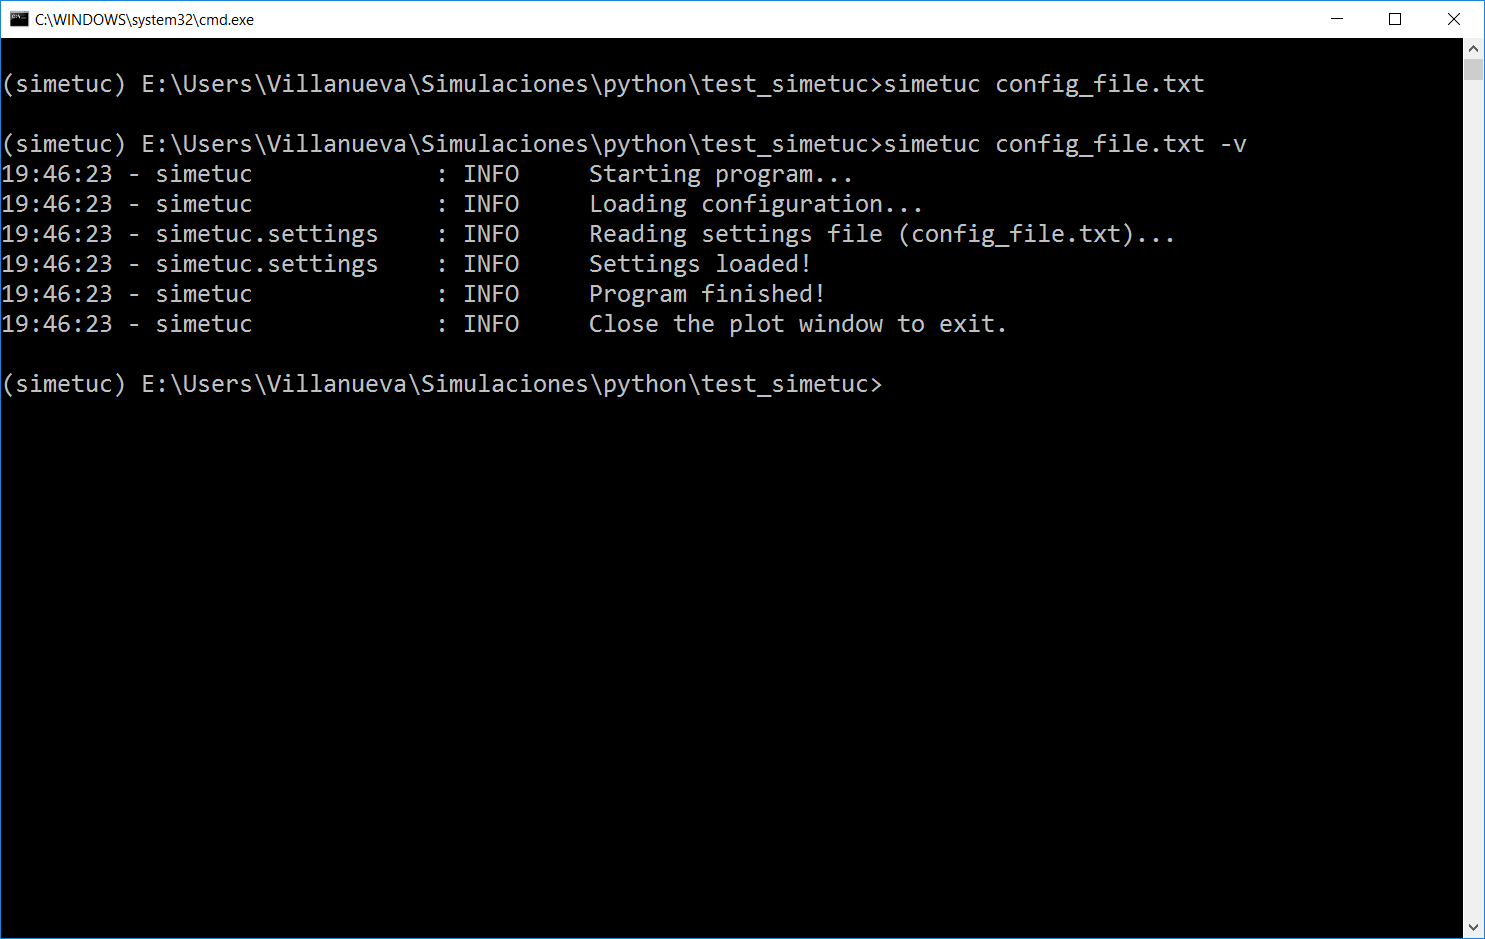
\includegraphics[width=1.2\columnwidth]{figures/correct_config_file.PNG}
\par\end{centering}
\caption{\label{fig:Example-conf_file_correct}Example of a correct configuration
file check with and without the verbose option.}
\end{figure}

\begin{figure}
\begin{centering}
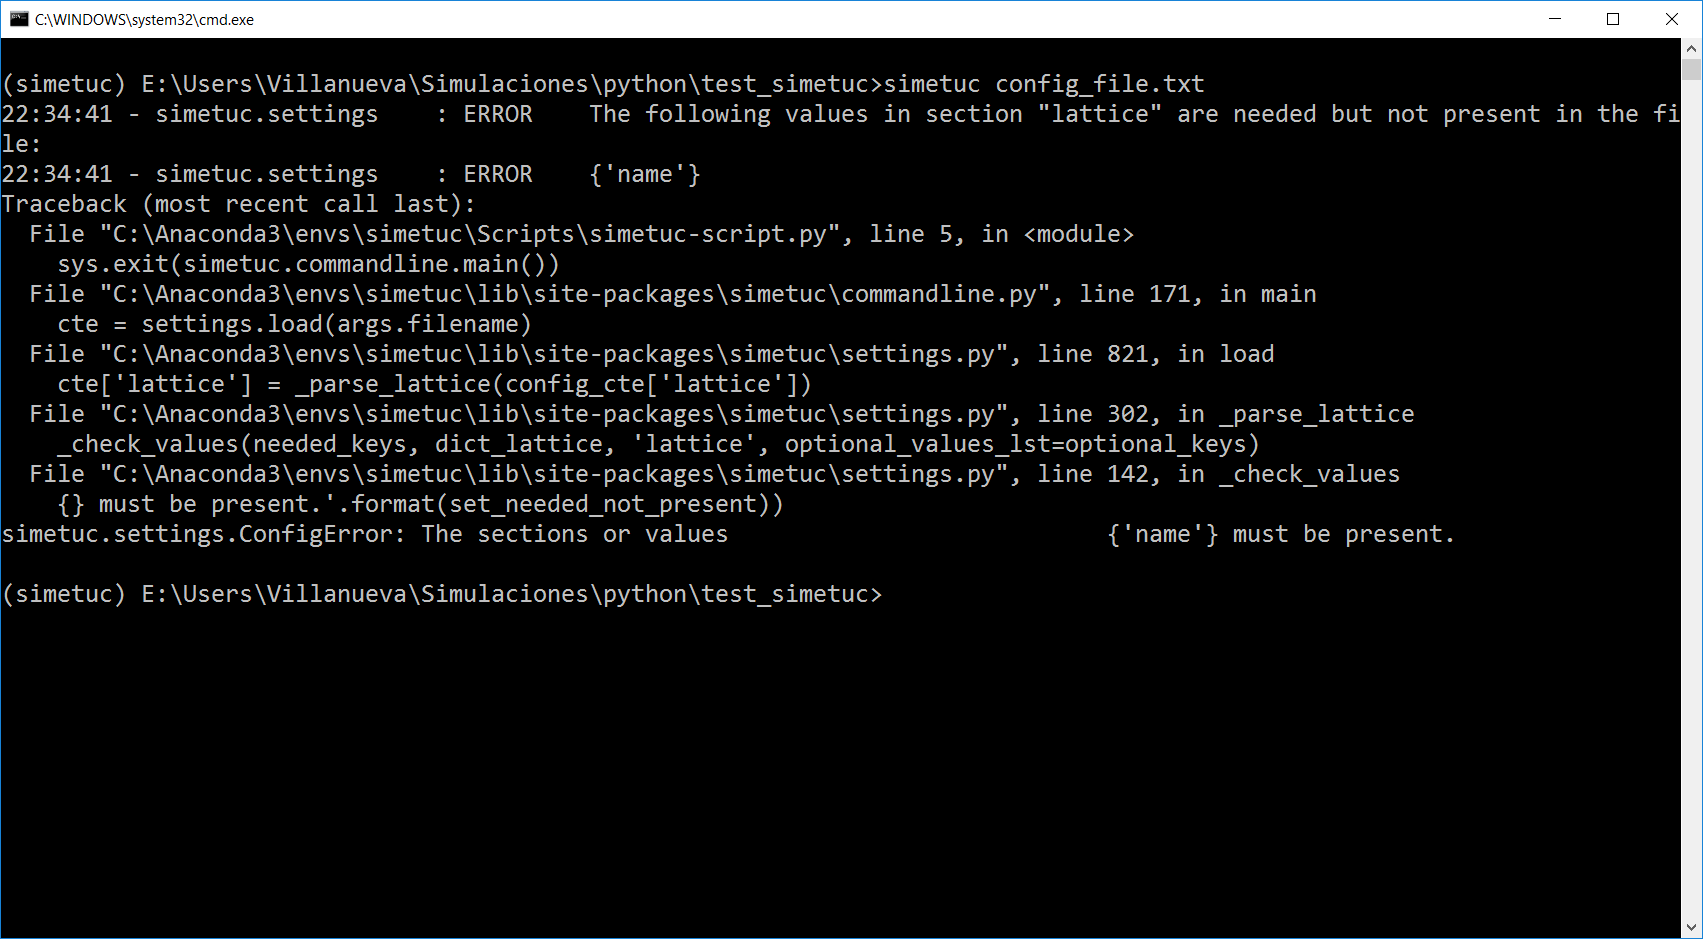
\includegraphics[width=1.2\columnwidth]{figures/config_file_wrong_lattice.PNG}
\par\end{centering}
\caption{\label{fig:Example-conf_file_wrong}Example of a wrong configuration
file check. The two upper lines show the user-friendly error message;
they can also be found in the error log (see Section \ref{subsec:Error-logs}).
In this case the name of the lattice was omitted from the file.}
\end{figure}


\chapter{The logs and results folders}

\emph{simetuc} creates several subfolders during its usage; these
subfolders are located under the current working directory (the directory
from which \emph{simetuc} is being used). Additionally, the experimental
data must be saved in a folder with a specific format, see Section
\ref{subsec:The-expData-folder}.

\section{The log folder}

Any operation of \emph{simetuc} writes its status and current tasks
on several log files, so the user can analyze what operations were
performed, when, and whether they succeeded. The log files are stored
in a subfolder called \texttt{logs}, which is created if it doesn't
exist.

\subsection{Normal log}

This is the primary log. Here all parts of the program register their
operations. For example, any operation begins with:

\begin{lstlisting}
2017-01-10 19:13:51,227 - simetuc       : INFO     Starting program...
\end{lstlisting}

The log format is the following:

\begin{lstlisting}
YYYY-MM-DD HH:MM:SS,mmm - simetuc[.part]   : LEVEL    message
\end{lstlisting}

The main program emits messages under the name \emph{simetuc}, other
parts of the program have names such as \emph{simetuc.lattice} or
\emph{simetuc.simulations}. The log level can be \texttt{DEBUG}, \texttt{INFO},
\texttt{WARNING}, or \texttt{ERROR}.

\subsection{\label{subsec:Error-logs}Error log}

Whenever an operation was requested, but couldn't be completed due
to an user error or an internal bug, the errors are written to an
error log. This is log remains empty if all operations succeeded.

\subsection{Debug log}

This log registers a lot of low level information that is usually
not important, but can be relevant in the case of errors.

\section{The results folder\label{sec:The-results-folder}}

All simulations produce some results that are stored in the subfolder
\texttt{results/latticeName} with the hdf5 format.

\section{Other folders}

The lattice folder, Section \ref{subsec:The-latticeData-folder}.

The experimental data folder, see Section \ref{subsec:The-expData-folder}.

\section{The HDF5 format\label{sec:The-HDF5-format}}

This is a open binary format that can be open with many scientific
software such as Matlab or Origin. A lightweight viewer is \href{https://support.hdfgroup.org/projects/compass/}{HDFCompass}.

\chapter{Simulations}

\section{Creating a lattice\label{sec:Creating-a-lattice}}

This is the first step in any simulation. The lattice and states section
of the configuration file determine the position of the doped ions
and the number of energy states.

The option for creating lattice is \texttt{-l}:

\begin{lstlisting}
simetuc config_file.txt -l
\end{lstlisting}

When given with the \texttt{-v} option to show the progress information,
the results look like Figure \ref{fig:Lattice-creation}.

\begin{figure}
\begin{centering}
\subfloat[]{\begin{centering}
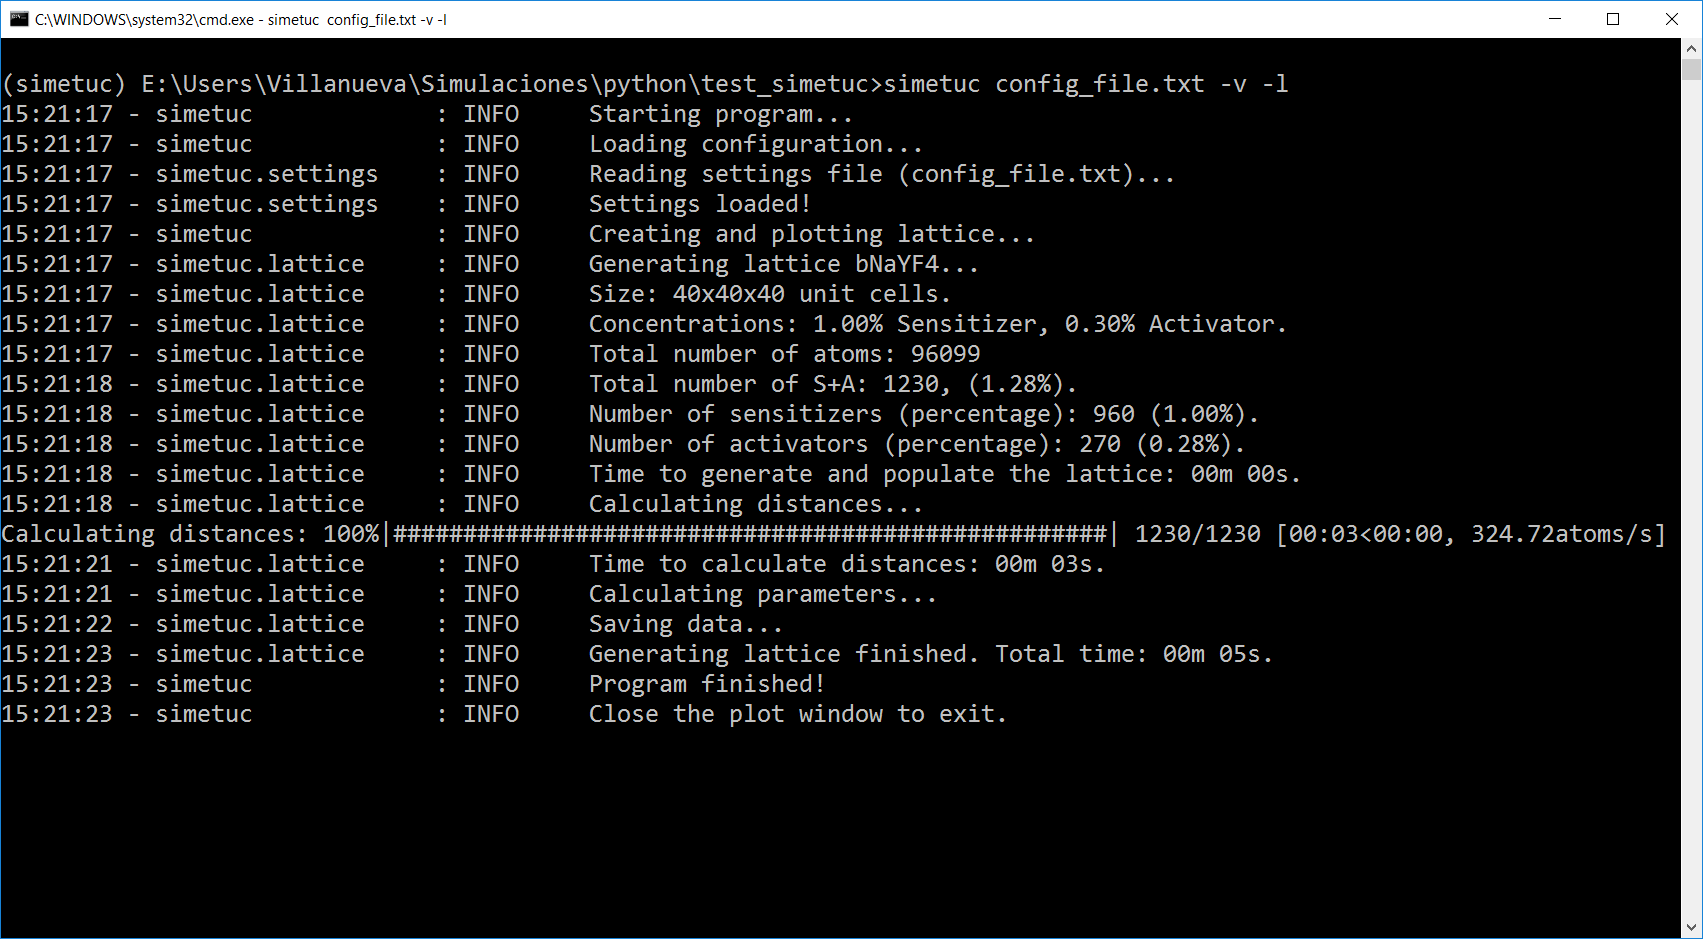
\includegraphics[width=1.2\textwidth]{figures/lattice_cmd.PNG}
\par\end{centering}
}
\par\end{centering}
\begin{centering}
\subfloat[]{\begin{centering}
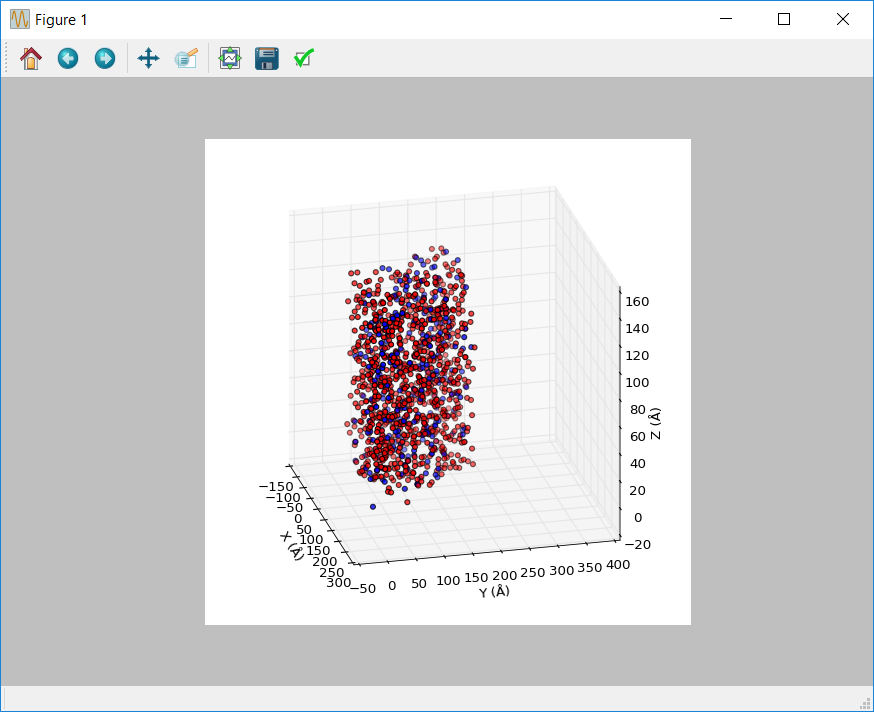
\includegraphics[width=1\columnwidth]{figures/lattice_plot.PNG}
\par\end{centering}
}\caption{\label{fig:Lattice-creation}Lattice creation. (a) shows the result
of invoking the command \texttt{simetuc config\_file.txt -v -l}. (b)
shows the positions of the doped ions, the sensitizers as red dots
and the activators as blue dots.}
\par\end{centering}
\end{figure}


\subsection{The \texttt{latticeData} folder\label{subsec:The-latticeData-folder}}

All created lattices are stored in a folder with the name of the lattice
under the latticeData subfolder; the name of the lattice is given
by the user in the configuration file, see Section \ref{subsec:Lattice}.
These saved files are used in subsequent simulations. The name format
under which they are saved is

\begin{lstlisting}
data_XXuc_y.yS_z.zA.hdf5
\end{lstlisting}

where $XX$ is the number of unit cells, $y.y$ is the concentration
of sensitizers and $z.z$ that of activators (both in percentage).

The file format is HDF5, see Section \ref{sec:The-HDF5-format}.

\section{Simulating the dynamics\label{sec:Simulating-the-dynamics}}

The simulation of the dynamics of a sample consists of two parts,
the excitation pulse and the subsequent relaxation. The dynamics simulation
includes the excitation, decay, branching ratios, and energy transfer
sections of the configuration file. The output is a plot of the average
decay curve of each state of the sensitizer and activator. The results
are saved to a file, see Section \ref{sec:The-results-folder}.

The option for simulating the dynamics is \texttt{-d}:

\begin{lstlisting}
simetuc config_file.txt -d
\end{lstlisting}

When given with the \texttt{-v} option to show the progress information,
the results look like Figure \ref{fig:Dynamics-simulation}.

\begin{figure}
\begin{centering}
\subfloat[]{\begin{centering}
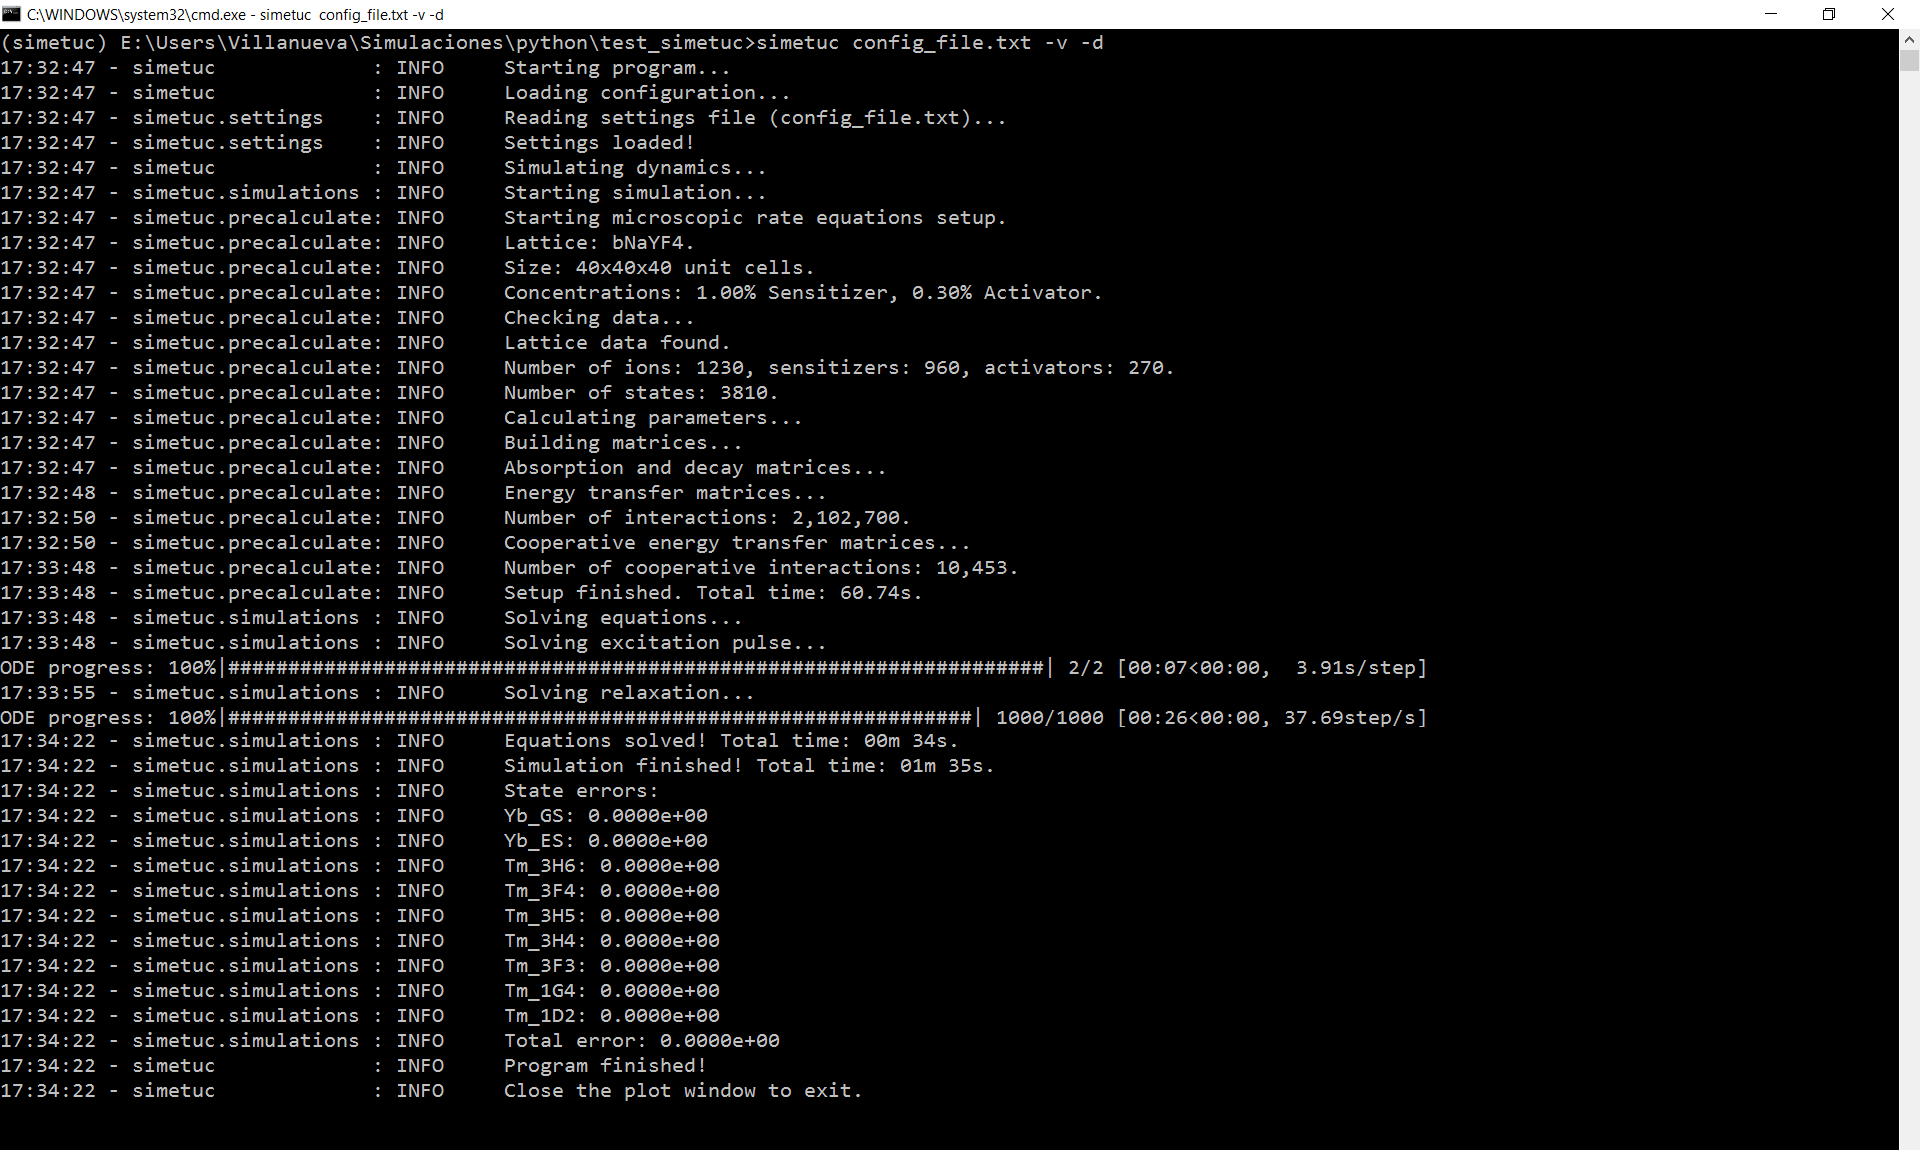
\includegraphics[width=1.2\textwidth]{figures/dynamics_cmd.PNG}
\par\end{centering}
}
\par\end{centering}
\centering{}\subfloat[]{\begin{centering}
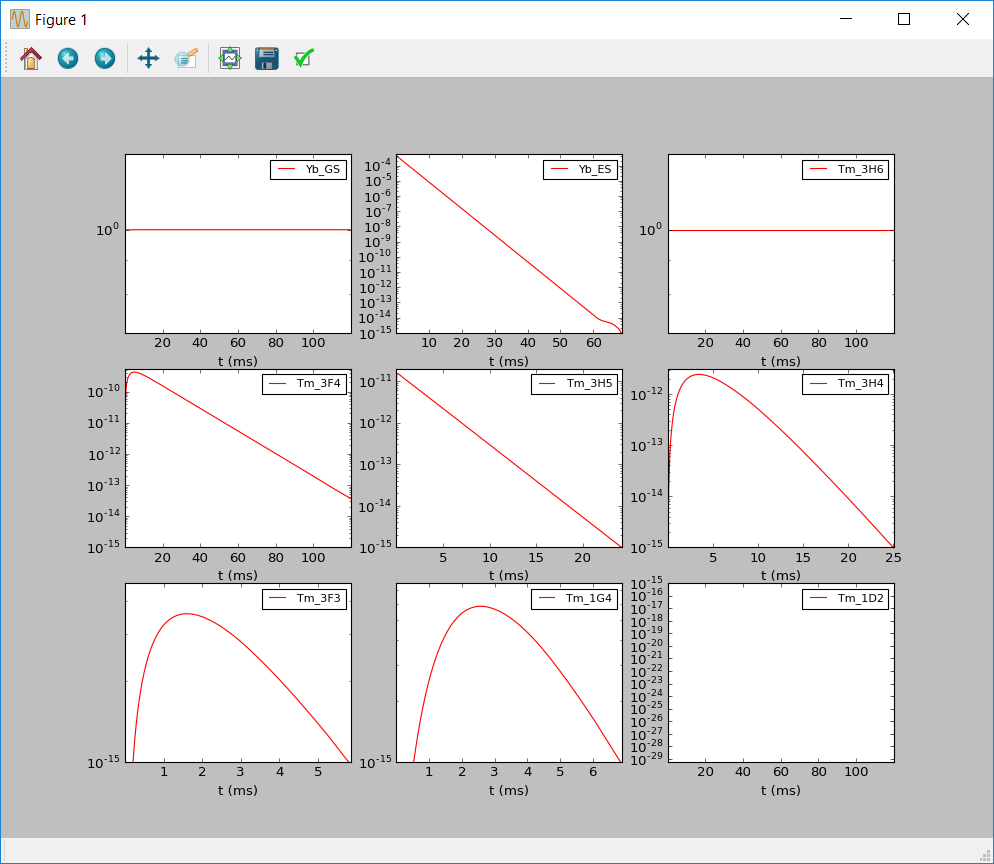
\includegraphics[width=1\columnwidth]{figures/dynamics_plot.PNG}
\par\end{centering}
}\caption{\label{fig:Dynamics-simulation}Dynamics simulation. (a) shows the
result of invoking the command \texttt{simetuc config\_file.txt -v
-d}. (b) shows a plot with the decay curves of all states of the sensitizer
and activator.}
\end{figure}


\section{Adding experimental data}

The comparison of the experimental to the simulated data is important
if to ensure that the energy transfer processes and their strengths
truly represent an accurate picture of the sample's behavior.

Decay experimental data is automatically loaded from the expData folder
(see next section), normalized and compared to the simulated decay
curve of the appropriate states. The deviation between the experimental
data and simulation is calculated for each level, and then all state
errors are added together to yield the total error.

\subsection{The \texttt{expData} folder\label{subsec:The-expData-folder}}

This folder should contain a subfolders with the name of the lattice.
Inside that subfolder several text files can be stored, each corresponding
to an ion's state decay for a given concentration of sensitizers and
activators. The name format is:

\begin{lstlisting}
decay_ION_STATE_exc_EXCLABEL_x.xION-S_y.yION-A.txt
\end{lstlisting}

where \texttt{ION}, \texttt{STATE}, and \texttt{EXCLABEL} are labels
defined in the configuration file: \texttt{ION} is an ion label, \texttt{STATE}
is an state label corresponding to \texttt{ION}, and \texttt{EXCLABEL}
is an excitation label defined in the excitations section of the configuration
file, see Section \ref{subsec:Excitation}. $x.x$ and $y.y$ are
the sensitizer (\texttt{ION-S}) and activator (\texttt{ION-A}) concentrations.

As an example, the decay curve of the Tm$^{3+}$ state $^{1}$D$_{2}$
for the \textgreek{b}-NaYF$_{4}$: 0.3\% Tm$^{3+}$ sample has a name:

\begin{lstlisting}
decay_Tm_1D2_exc_Vis_473_0.0Yb_0.3Tm.txt
\end{lstlisting}

and is stored in the folder \texttt{expData/bNaYF4}.

The experimental data files must have two columns separated by spaces
or tabs:
\begin{enumerate}
\item The first one with the time in seconds.
\item The second one with the emission intensity in any units (it will be
normalized).
\end{enumerate}
Lines starting with \texttt{\#} are ignored as comments. For example:

\begin{lstlisting}
# tau_em360_NYF_03Tm_EKSPLA473 
# time in seconds
0			0.405264768901133
1.99999999999978E-7	0.42944597490052
3.99999999999956E-7	0.432506887052342
5.99999999999989E-7	0.43954698500153
7.99999999999967E-7	0.4640342822161
1E-6			0.468931741659014
1.19999999999998E-6	0.498010407101316
1.39999999999996E-6	0.48852157943067
1.59999999999999E-6	0.51147842056933
1.79999999999997E-6	0.513927150290787
...
\end{lstlisting}

Once the experimental data files are in the right folder and with
the right names, they will be loaded automatically, like shown in
Figure \ref{fig:Dynamics-simulation-with-expdata}. The state and
total errors will be shown in the commandline and recorded in the
log files.

\begin{figure}
\begin{centering}
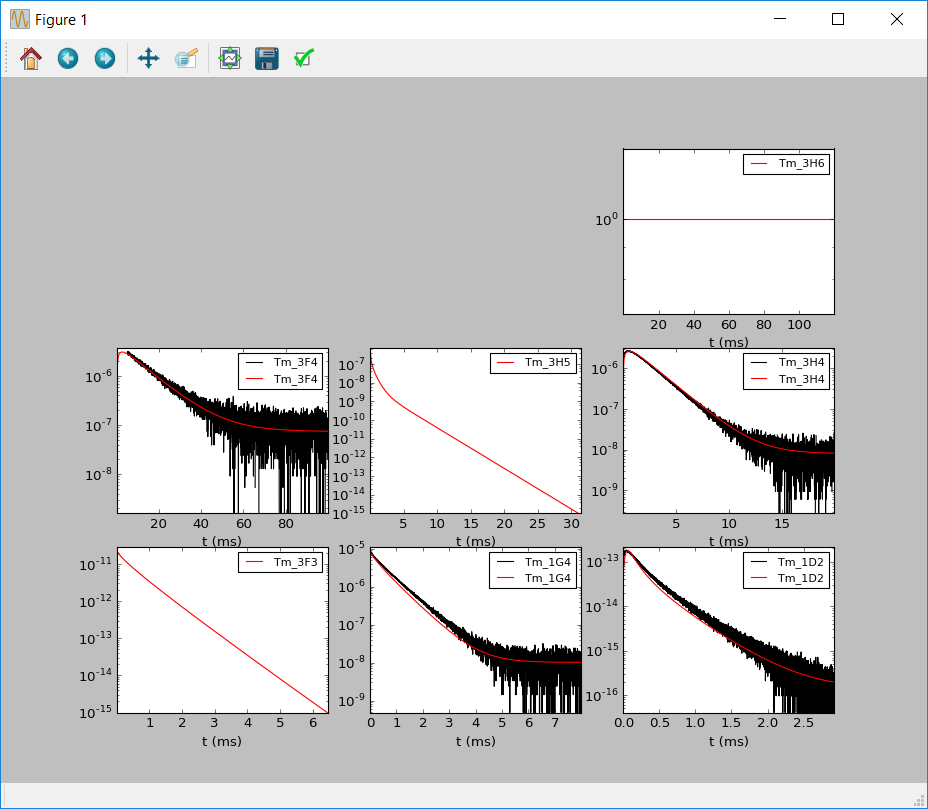
\includegraphics[width=1\textwidth]{figures/dynamics_plot_expData.PNG}
\par\end{centering}
\caption{\label{fig:Dynamics-simulation-with-expdata}Dynamics simulation with
experimental data.}

\end{figure}


\section{Optimizing the ET parameters\label{sec:Optimizing-the-ET-params}}

The strength of the interactions is \textit{a priori} unknown, but,
by fitting the simulations to the experimental data, it is possible
to obtain realistic interaction strengths.

The option for optimizing the dynamics is \texttt{-o}:

\begin{lstlisting}
simetuc config_file.txt -o
\end{lstlisting}

When given with the \texttt{-v} option to show the progress information,
the results look like Figure \ref{fig:Optimization-of-the}. The total
error has decreased from $0.2202$ to $0.1868$ when the energy transfer
parameters changed from $\unit[1.3\,10^{9}]{s^{-1}\,\AA^{6}}$ to
$\unit[2.4\,10^{9}]{s^{-1}\,\AA^{6}}$ for the parameter \texttt{CR50}
and from $\unit[1.5\,10^{9}]{s^{-1}\,\AA^{6}}$ to $\unit[4.1\,10^{9}]{s^{-1}\,\AA^{6}}$
for the parameter \texttt{ETU53}.

The optimization procedure does not change the configuration file
(\emph{simetuc} never does), so the parameter values should be changed
by the user. It is advisable to re-run a dynamics simulation with
the new parameters to check that the fit is satisfactory.

When optimizing a system for the first time it is recommended to first
use the \texttt{brute\_force} method, update the configuration file
with its results, and then run the optimization again with the \texttt{SLSQP}
method, see Section \ref{subsec:Optimization-Method}.

\begin{figure}
\begin{centering}
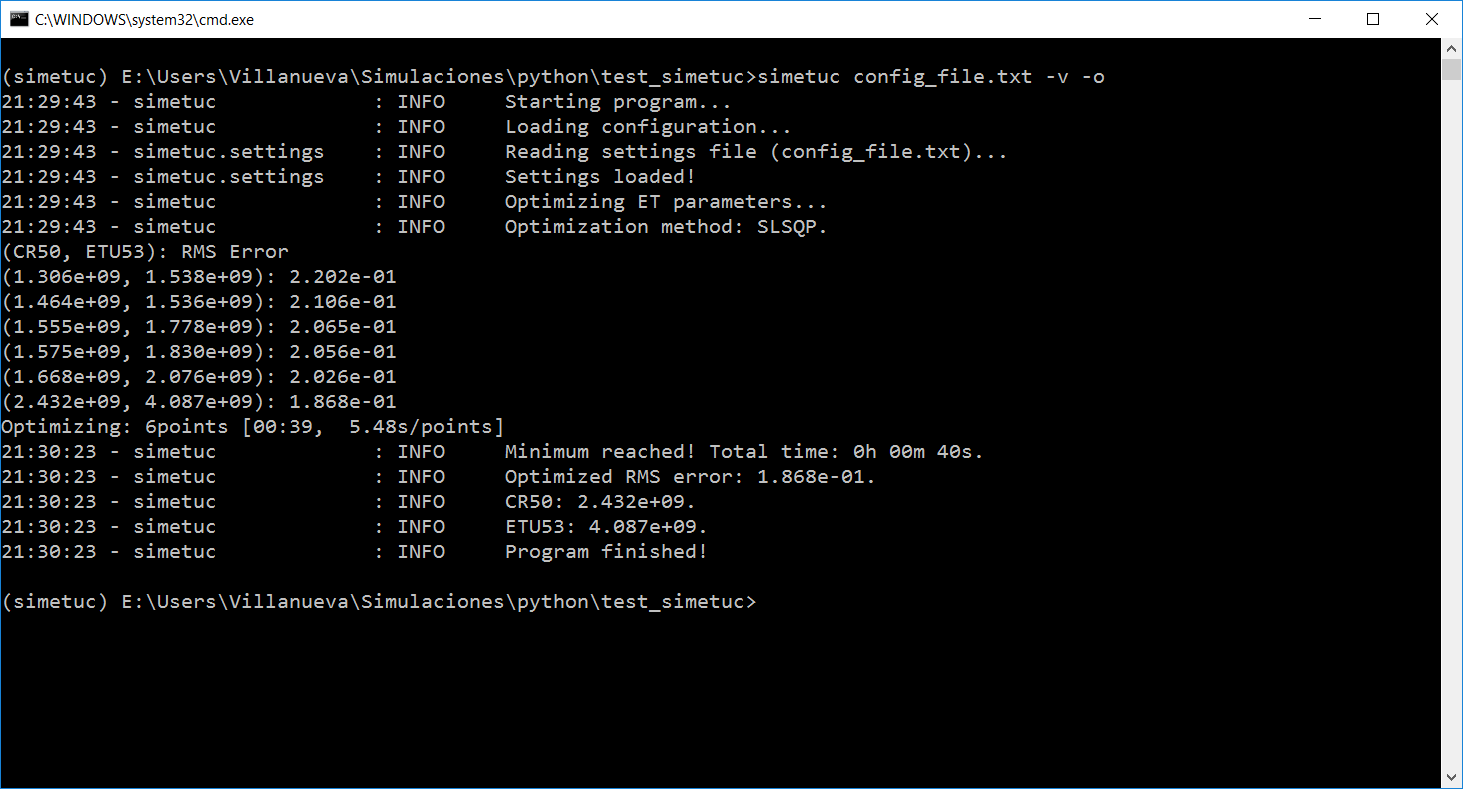
\includegraphics[width=1.2\textwidth]{figures/optimize_cmd.PNG}
\par\end{centering}
\caption{\label{fig:Optimization-of-the}Optimization of the dynamics with
the command \texttt{simetuc config\_file.txt -v -o}.}

\end{figure}


\section{Simulating the steady state\label{sec:Simulating-the-steady-state}}

If the excitation source is not pulsed, but it is kept switched on
continuously, the states will reach a steady state; that is, the states
will have a population that does not change anymore with time. The
time it takes for the system to reach the steady state depends on
the lifetimes and energy transfer processes.

The steady state populations are proportional to the emission intensity
of each state under continuous excitation.

The excitation source activated in the configuration file should have
a realistic excitation power density; usually pulsed sources have
much higher instantaneous powers, see Section \ref{subsec:Excitation}.

The option for simulating the steady state is \texttt{-s}:

\begin{lstlisting}
simetuc config_file.txt -s
\end{lstlisting}

When given with the \texttt{-v} option to show the progress information,
the results look like Figure \ref{fig:Steady-state-simulation}.

\begin{figure}
\begin{centering}
\subfloat[]{\begin{centering}
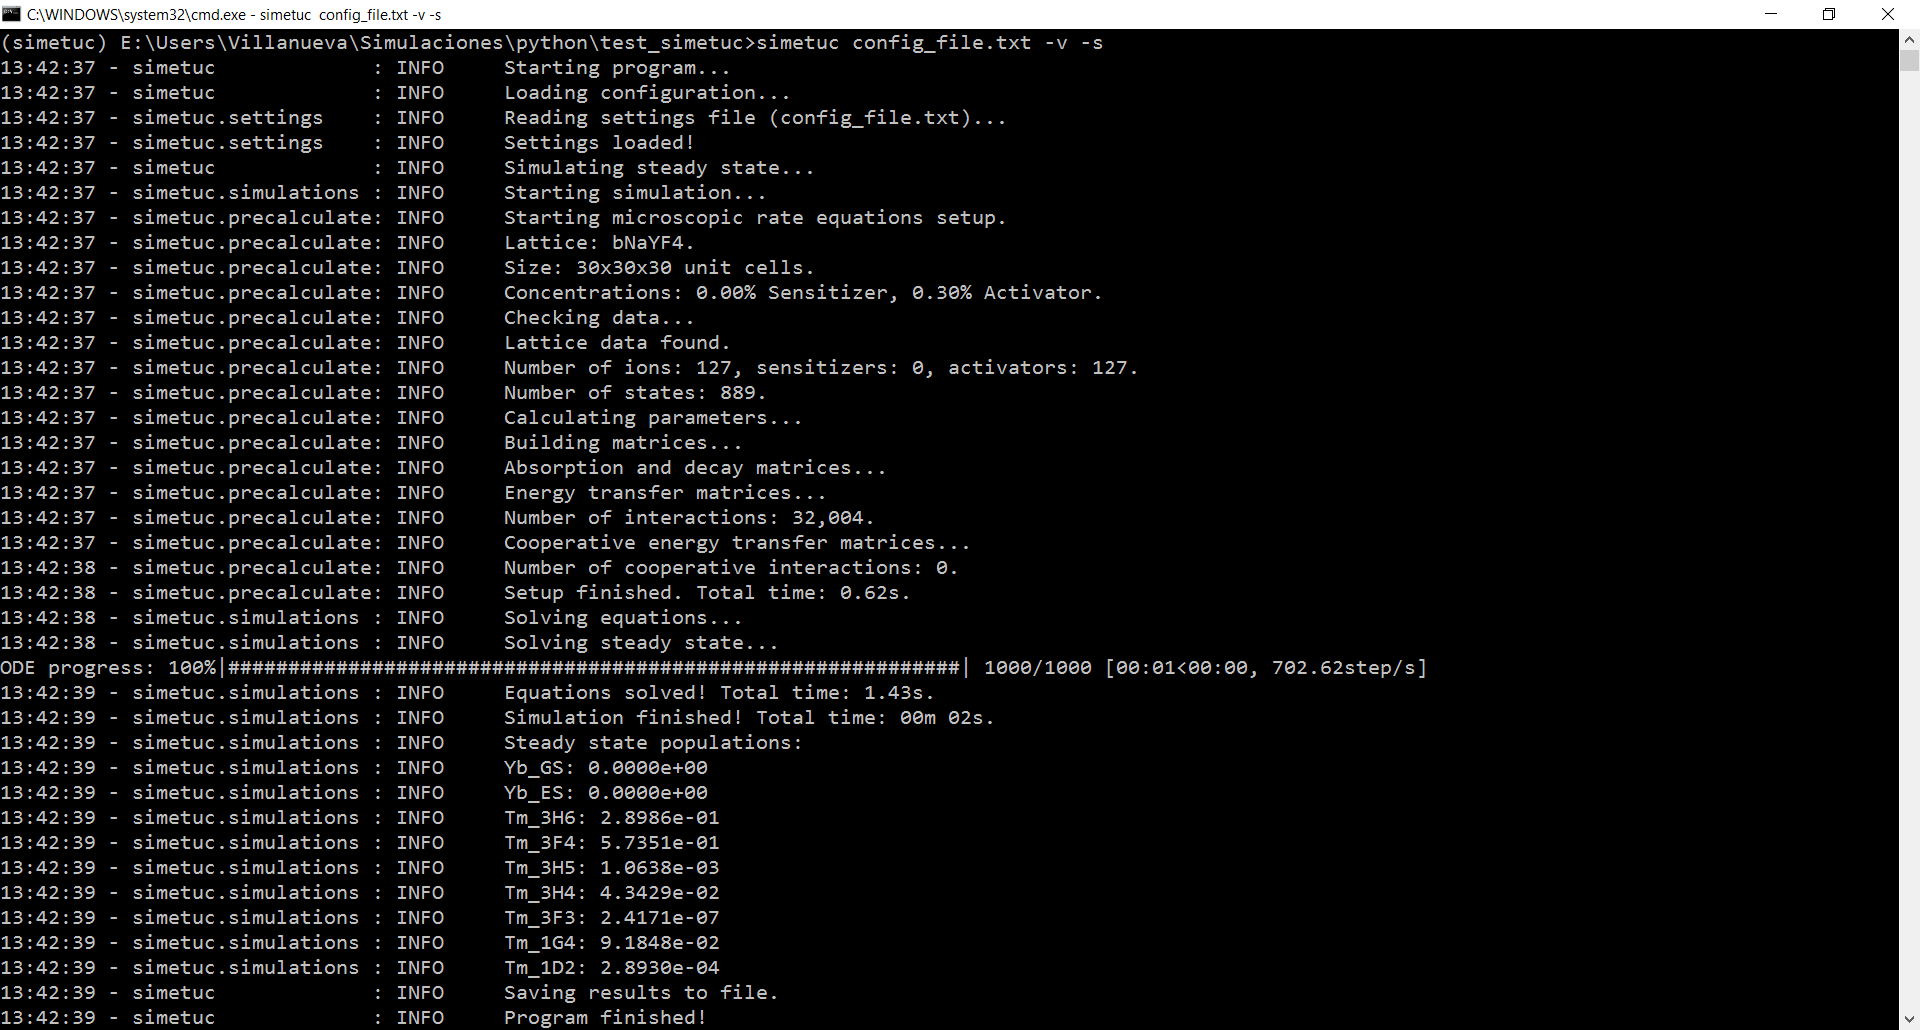
\includegraphics[width=1.2\textwidth]{figures/steady_state_cmd.PNG}
\par\end{centering}
}
\par\end{centering}
\centering{}\subfloat[]{\begin{centering}
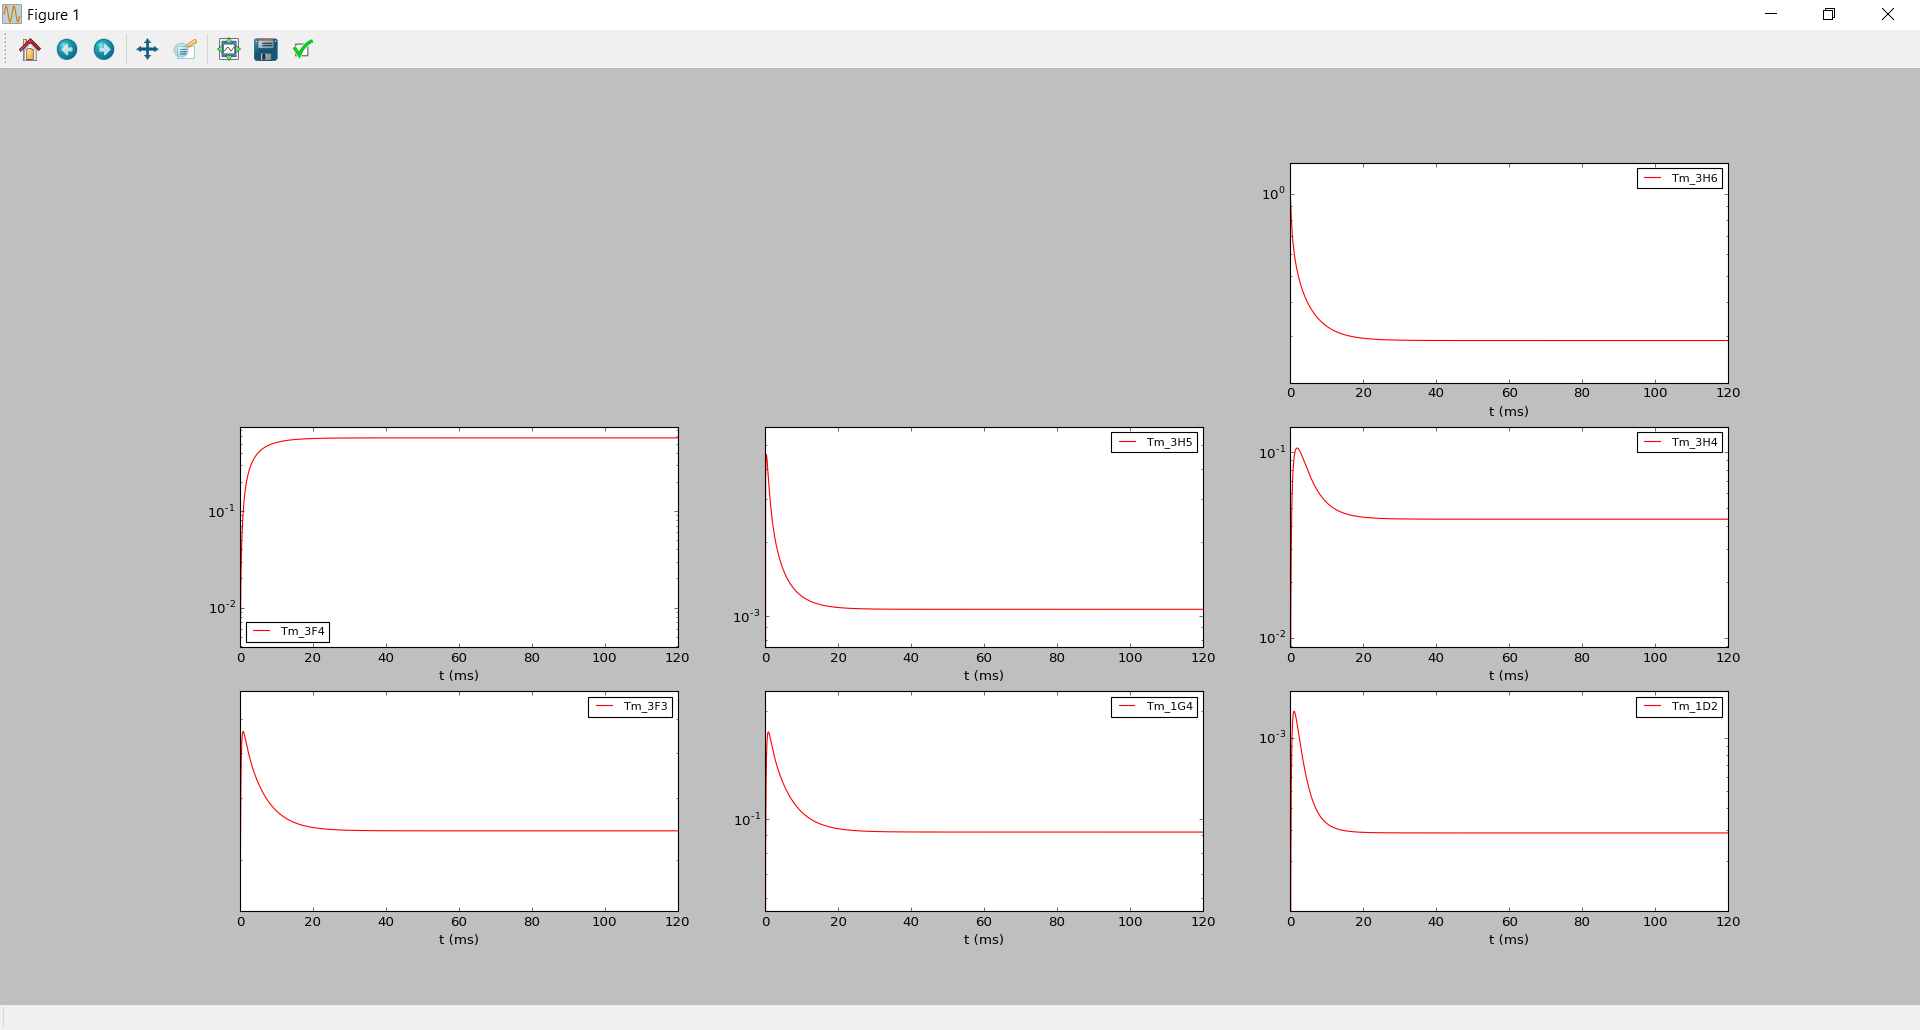
\includegraphics[width=1\columnwidth]{figures/steady_state_plot.PNG}
\par\end{centering}
}\caption{\label{fig:Steady-state-simulation}Steady state simulation. (a) shows
the result of invoking the command \texttt{simetuc config\_file.txt
-v -s}. (b) shows a plot with the decay curves of all states of the
sensitizer and activator. All states have reached their steady state.}
\end{figure}


\section[Simulating the power dependence]{Simulating the power dependence of the steady state\label{sec:Simulating-the-power-dep}}

A standard upconversion experiment consists in measuring the emission
intensity (usually the area under the emission peak, but also just
the maximum) as a function of the excitation power. The power dependence
of the emission $I$ usually follows a power law: $I=P^{n}$, where
$P$ is the excitation power and $n$ is the number of photons involved
in the mechanism; this is an approximation that only works at low
excitation powers.

This simulations are capable of producing the entire power dependence
curve so it can be compared to the experimental one. \emph{simetuc}
simulates the steady state for the excitation powers defined in the
configuration file and shows the steady state populations in a log-log
plot. See Section \ref{subsec:Power-Dependence} for the configuration
file options.

The option for simulating the steady state is \texttt{-p}:

\begin{lstlisting}
simetuc config_file.txt -p
\end{lstlisting}

When given with the \texttt{-v} option to show the progress information,
the results look like Figure \ref{fig:Steady-state-simulation}.

\begin{figure}
\begin{centering}
\subfloat[]{\begin{centering}
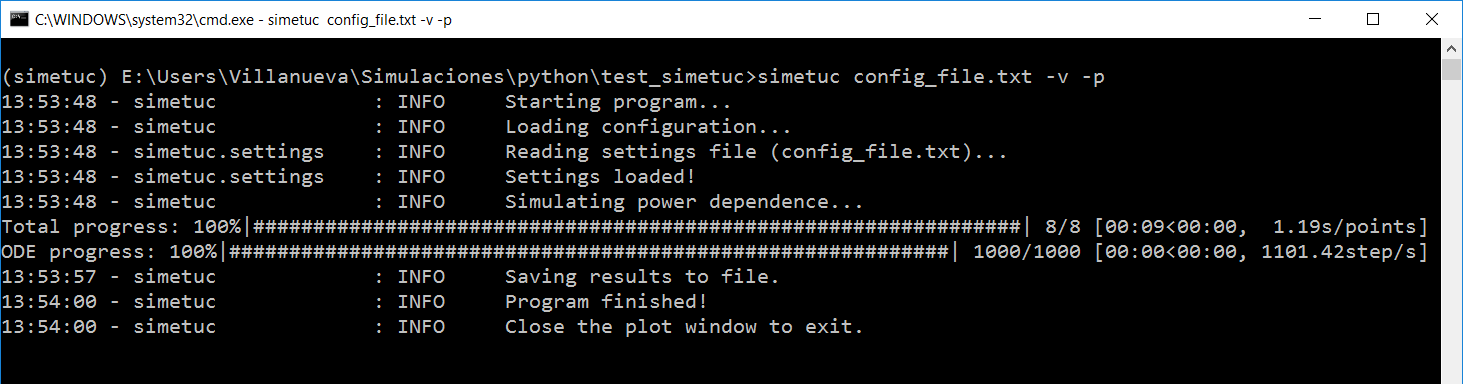
\includegraphics[width=1.1\textwidth]{figures/pow_dep_cmd.PNG}
\par\end{centering}
}
\par\end{centering}
\centering{}\subfloat[]{\begin{centering}
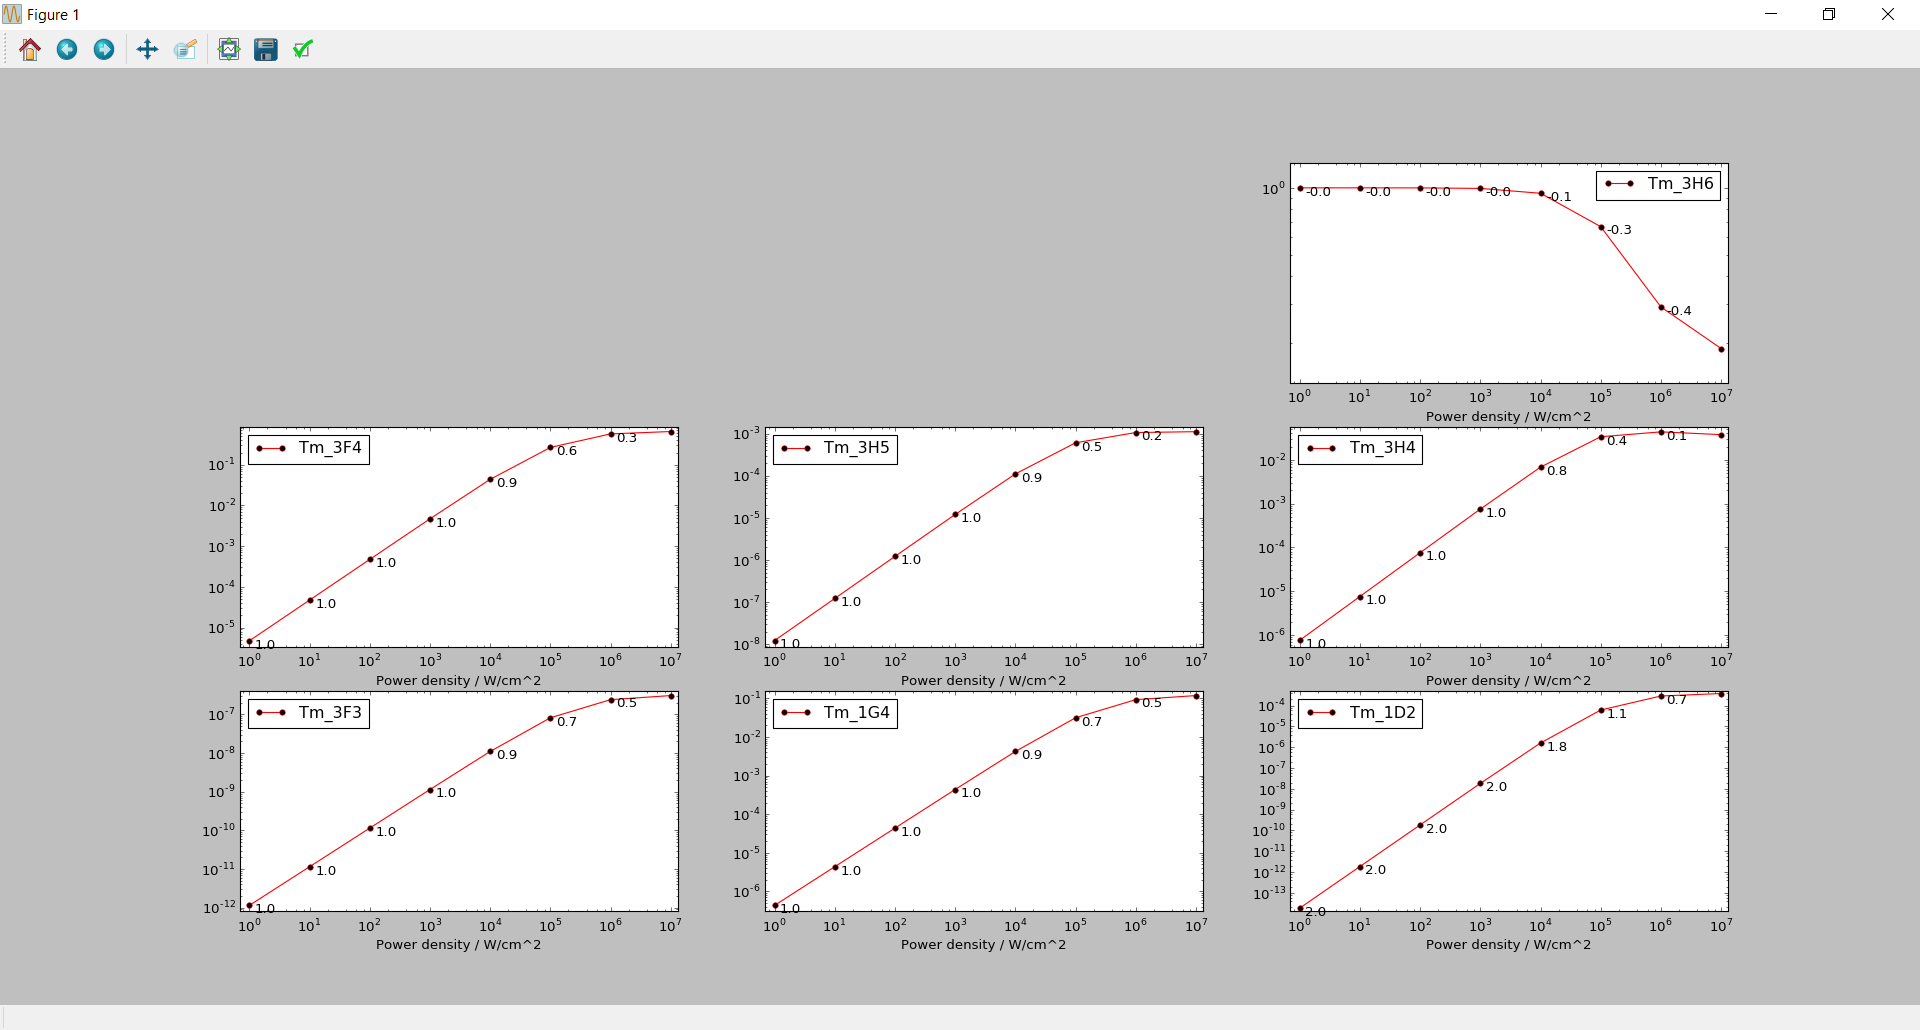
\includegraphics[width=1\columnwidth]{figures/pow_dep_plot.PNG}
\par\end{centering}
}\caption{\label{fig:Power-dependence}Power dependence simulation. (a) shows
the result of invoking the command \texttt{simetuc config\_file.txt
-v -p}. (b) shows a plot with the emission power dependence of all
states of the sensitizer and activator. The simulated excitation powers
are taken from the configuration file. In this case, unrealistically
high powers have been simulated to show the saturation regime.}
\end{figure}


\section[Simulating the concentration dependence]{Simulating the concentration dependence of the the steady state
or of the dynamics\label{sec:Simulating-the-concentration-dep}}

One of the strongest points of the microscopic rate equations that
\emph{simetuc} solves is that once the lifetimes, branching ratios
and energy transfer parameters are known, it is possible to change
the concentrations of sensitizers and activators and simulate the
decay curves or the steady state, thus predicting the behavior of
a new sample.

Simulating the concentration dependence of the steady state is equivalent
to simulate the emission efficiency of each state as a function of
both concentrations. Simulating the concentration dependence of the
dynamic is useful to compare it with experimental data, because decay
curves are easier to measure than emission efficiencies.

The simulated concentration range is controlled with the configuration
file, see Section \ref{subsec:Concentration-Dependence}. The option
for simulating the concentration dependence of the steady state is
\texttt{-c}:

\begin{lstlisting}
simetuc config_file.txt -c
\end{lstlisting}

When given with the \texttt{-v} option to show the progress information,
the results look like Figure \ref{fig:Conc-dependence}.

\begin{figure}
\begin{centering}
\subfloat[]{\begin{centering}
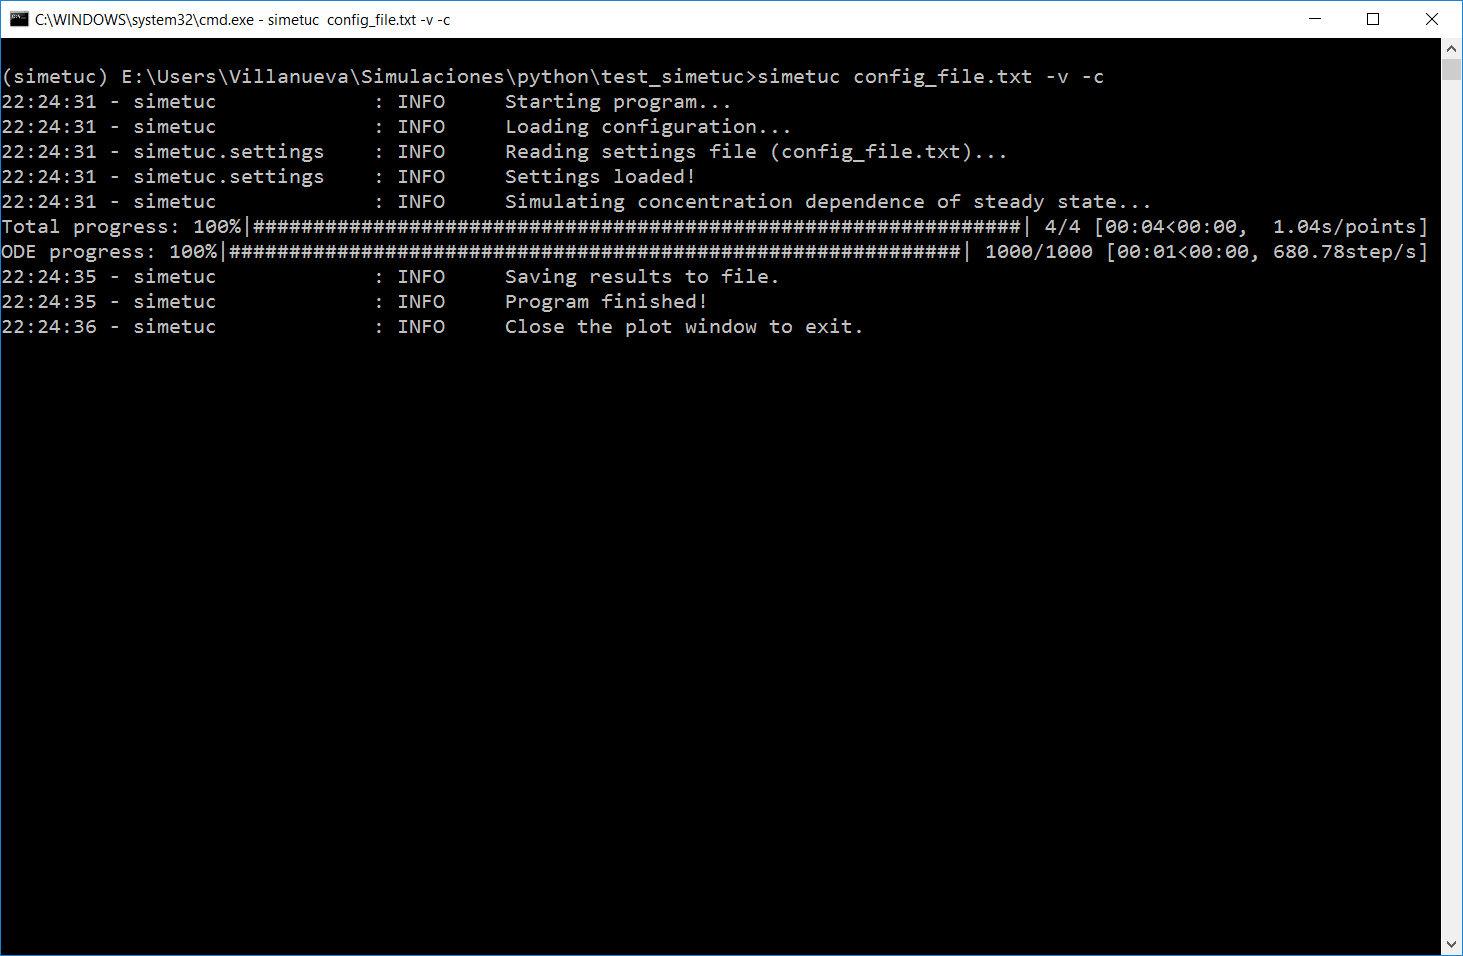
\includegraphics[width=1.2\textwidth]{figures/conc_dep_steady_cmd.PNG}
\par\end{centering}
}
\par\end{centering}
\begin{centering}
\subfloat[]{\begin{centering}
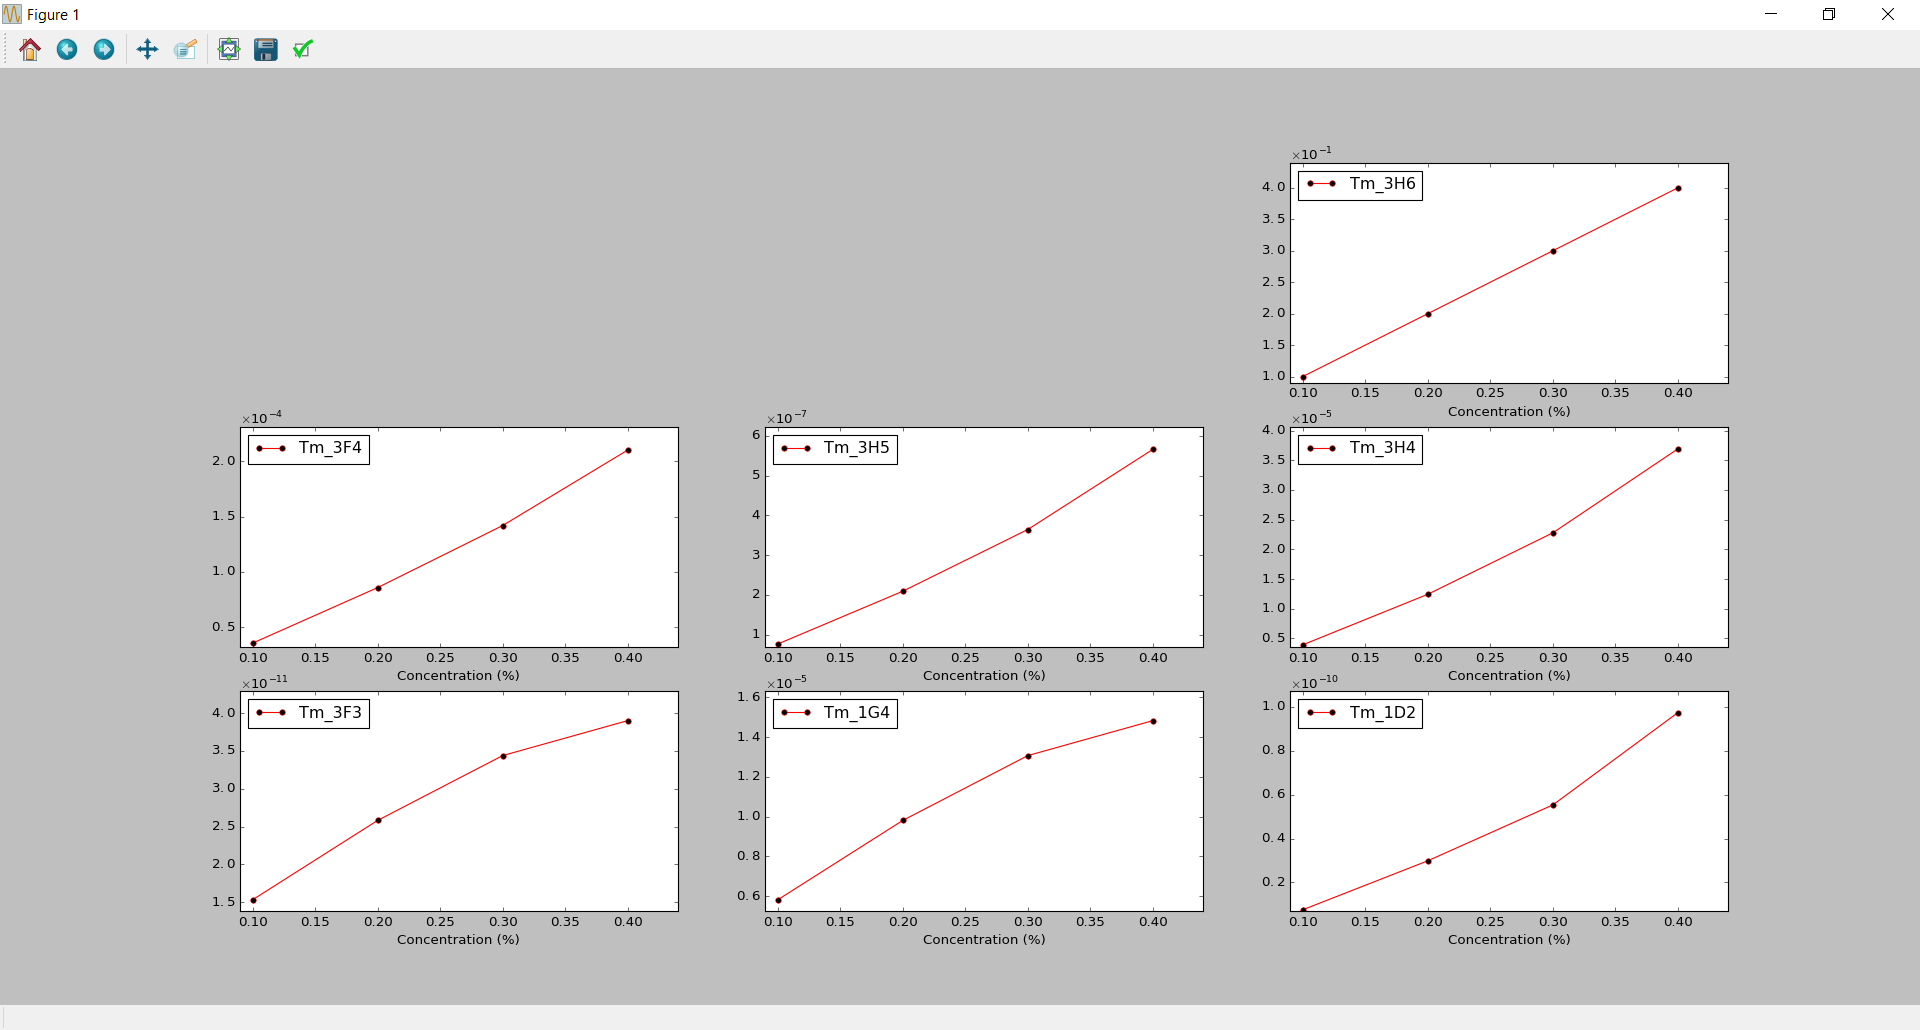
\includegraphics[width=1\columnwidth]{figures/conc_dep_steady_plot.PNG}
\par\end{centering}
}
\par\end{centering}
\centering{}\subfloat[]{\begin{centering}
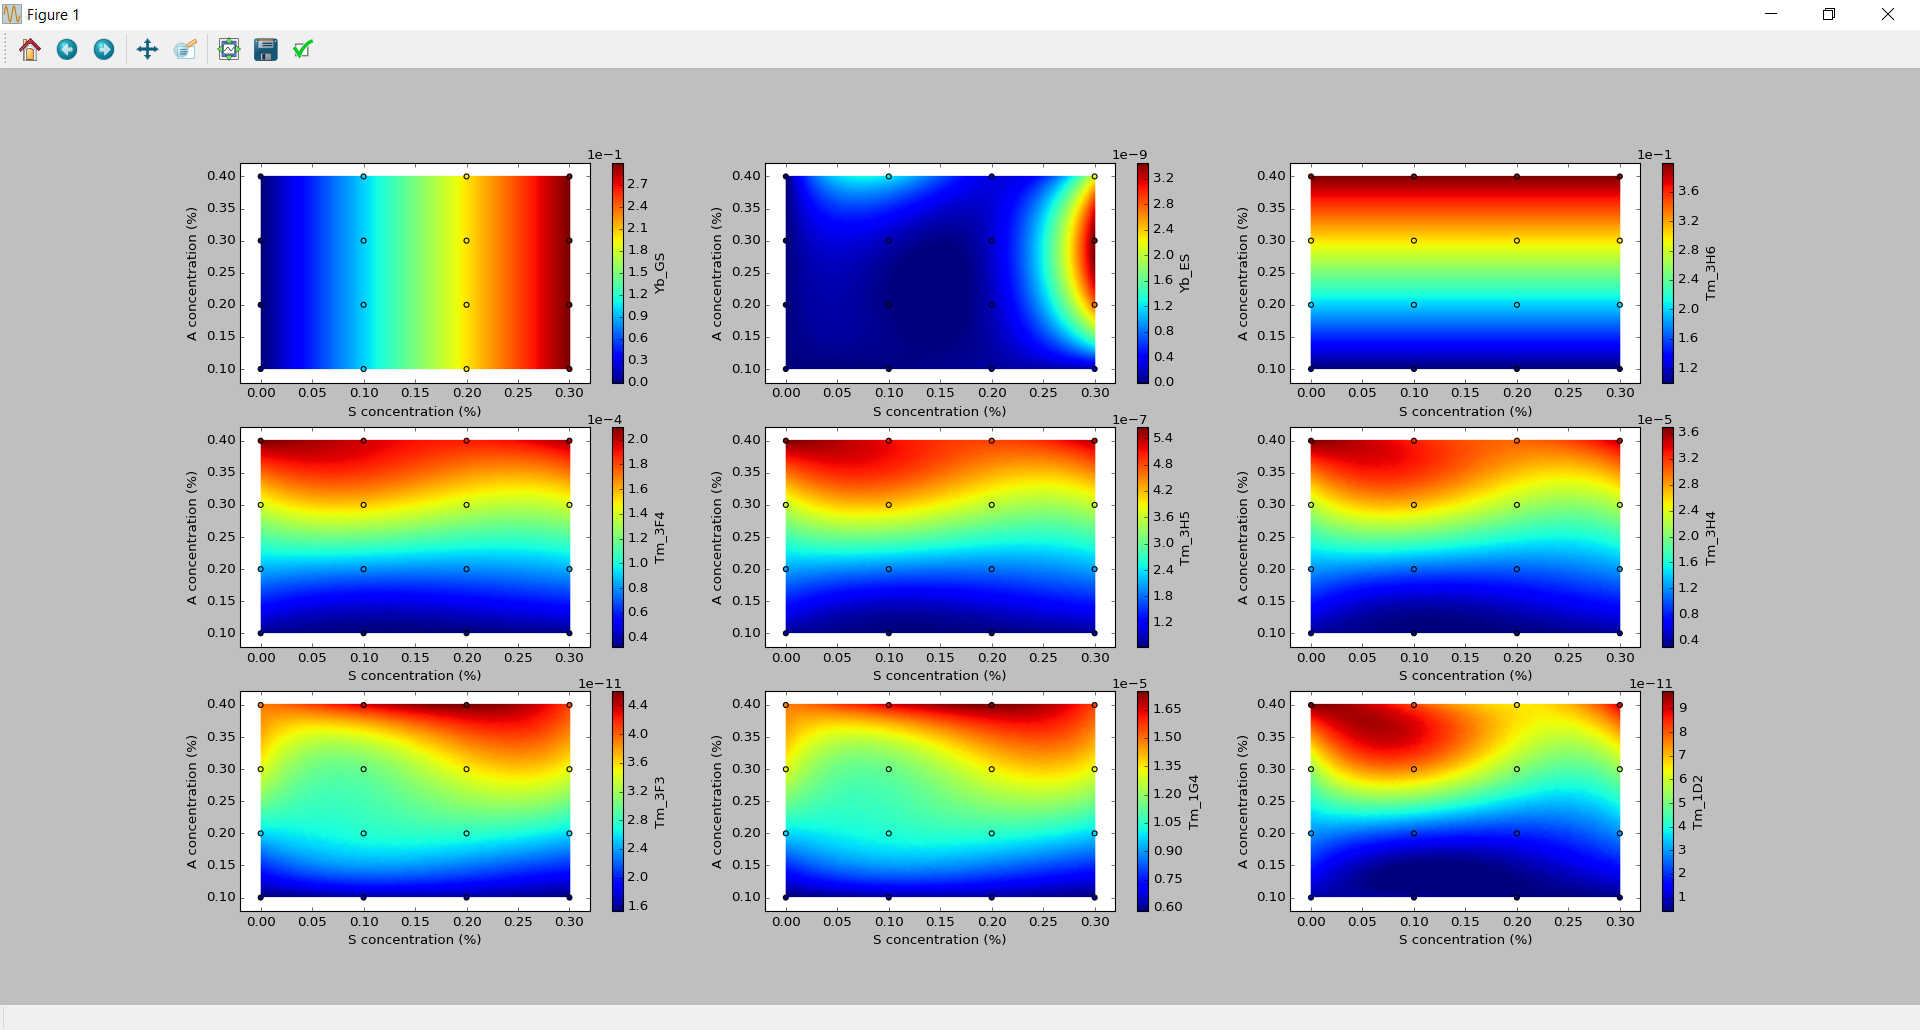
\includegraphics[width=1\columnwidth]{figures/conc_dep_steady_plot_2D.PNG}
\par\end{centering}
}\caption{\label{fig:Conc-dependence}Concentration dependence of the steady
state. (a) shows the result of invoking the command \texttt{simetuc
config\_file.txt -v -c}. (b) and (c) show plots with the concentration
dependence of the emission. The simulated concentrations are taken
from the configuration file. In (b) the sensitizer concentration is
fixed at 0\%, only the activator concentration changes. In (c) both
concentrations change.}
\end{figure}

The option for simulating the concentration dependence of the dynamics
is \texttt{-c d}:

\begin{lstlisting}
simetuc config_file.txt -c d
\end{lstlisting}

When given with the \texttt{-v} option to show the progress information,
the results look like Figure \ref{fig:Conc-dependence-dyn}.

\begin{figure}
\begin{centering}
\subfloat[]{\begin{centering}
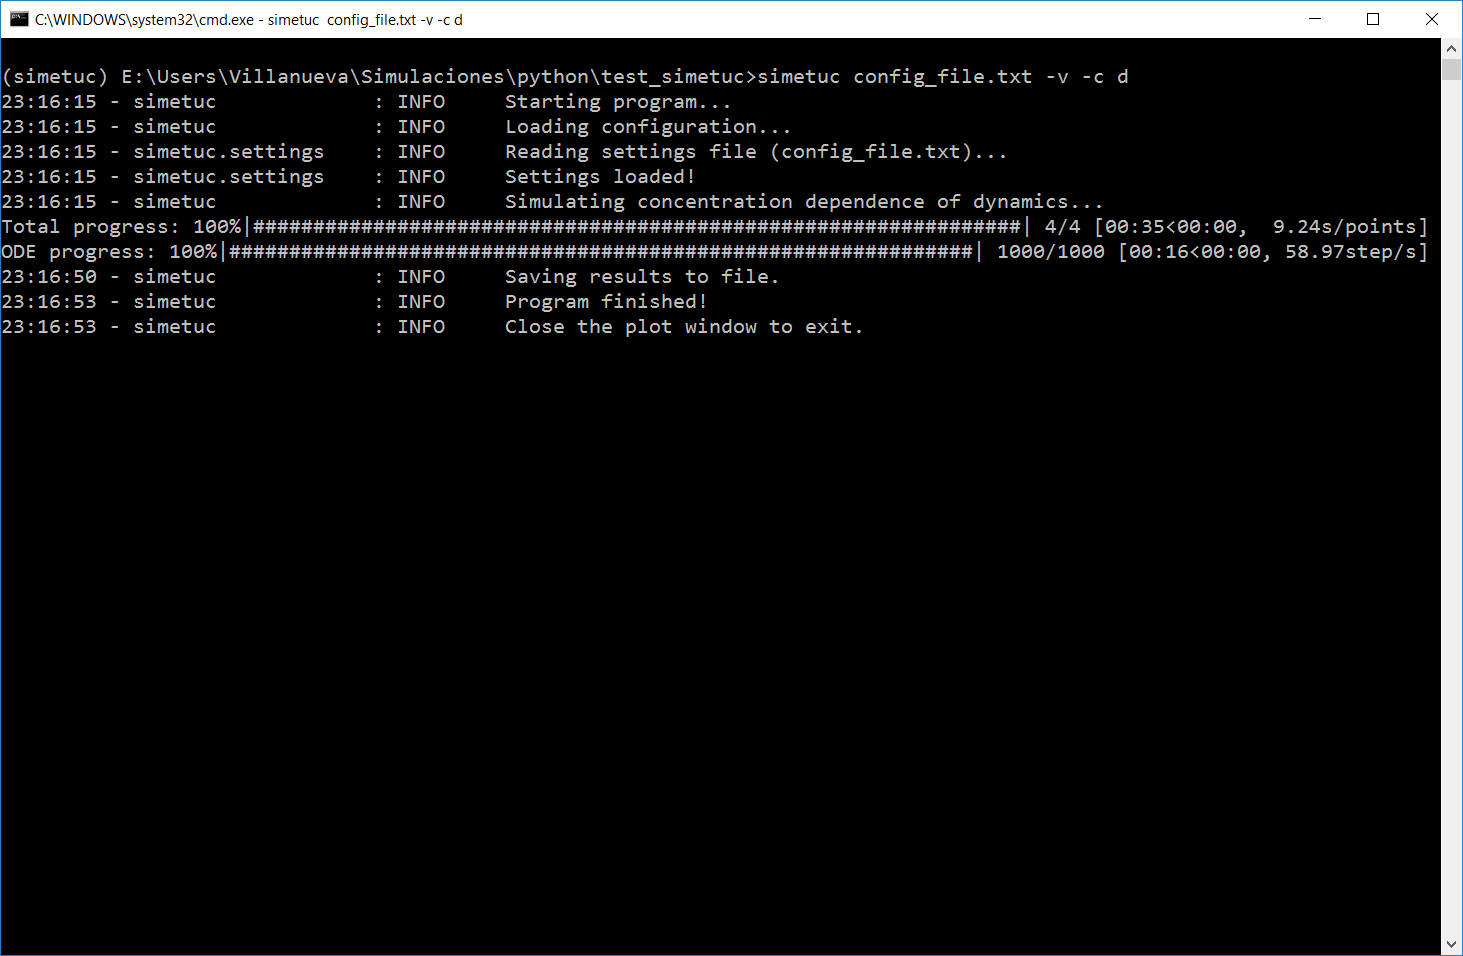
\includegraphics[width=1.1\textwidth]{figures/conc_dep_dyn_cmd.PNG}
\par\end{centering}
}
\par\end{centering}
\centering{}\subfloat[]{\begin{centering}
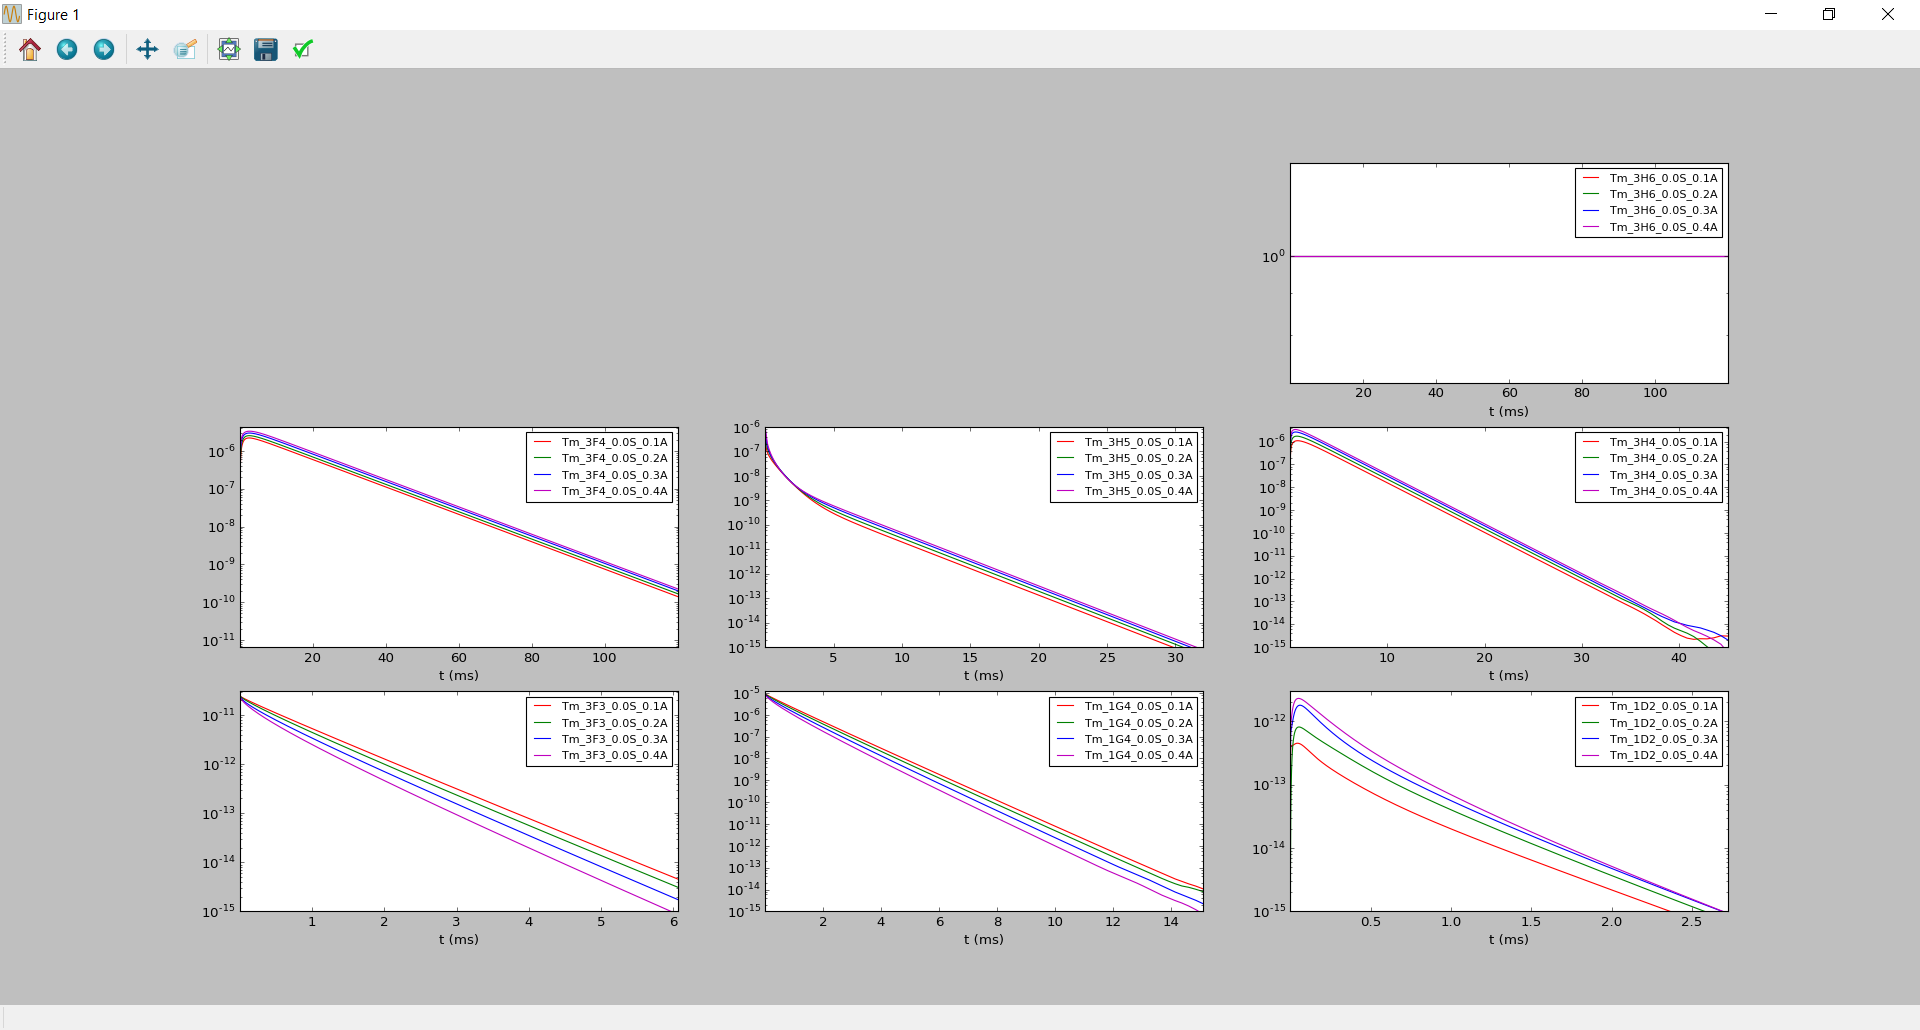
\includegraphics[width=1\columnwidth]{figures/conc_dep_dyn_plot.PNG}
\par\end{centering}
}\caption{\label{fig:Conc-dependence-dyn}Concentration dependence of the dynamics.
(a) shows the result of invoking the command \texttt{simetuc config\_file.txt
-v -c d}. (b) shows a plot with the decay curves at different concentrations.
The simulated concentrations are taken from the configuration file.}
\end{figure}


\section{Microscopic or average rate equations\label{sec:Microscopic-or-average}}

It is useful to compare the results of the microscopic rate equation
model to the standard average rate equation model. All simulations
can be performed with the average model using the \texttt{-{}-average}
flag in a command, for example

\begin{lstlisting}
simetuc config_file.txt -d --average
\end{lstlisting}
will simulate the dynamics using the average model and 
\begin{lstlisting}
simetuc config_file.txt -p --average
\end{lstlisting}

will simulate the power dependence of the average model.

In the average model, all sensitizer ions are represented as one average
ion (same for the activators), therefore all energy migration processes
are ignored (technically speaking, the average model has infinite
energy migration between all states).

The energy transfer parameters in the average model are not the microscopic
parameters between two ions, but an average of all interactions between
the ions in the sample, which are at different distances. This means
that knowledge of the average ET parameters for a sample with a certain
concentration does not give much information about the ET parameters
at other concentrations. That is, fitting decay data with the average
model gives limited information (average ET strengths) about that
sample and nothing about different samples.

\chapter{Publications and acknowledgments}

This software has been described and used in these publications:
\begin{itemize}
\item Villanueva-Delgado, P.; Kr�mer, K. W. \& Valiente, R. Simulating Energy
Transfer and Upconversion in \textgreek{b}-NaYF\textsubscript{4}:
Yb\textsuperscript{3+}, Tm\textsuperscript{3+}, \emph{J. Phys. Chem.
C}, \textbf{2015}, \emph{119} (41), pp 23648\textendash 23657. \href{http://pubs.acs.org/doi/10.1021/acs.jpcc.5b06770}{DOI: 10.1021/acs.jpcc.5b06770}.
\item Villanueva-Delgado, P.; Kr�mer, K. W.; Valiente, R.; de Jong, M. \&
Meijerink, A. Modeling Blue to UV Upconversion in \textgreek{b}-NaYF\textsubscript{4}:
Tm\textsuperscript{3+}, \emph{Phys. Chem. Chem. Phys.}, \textbf{2016},
\emph{18}, pp 27396-27404, \href{http://pubs.rsc.org/en/Content/ArticleLanding/2016/CP/C6CP04347J\#!divAbstract}{DOI: 10.1039/C6CP04347J}.
\item Villanueva-Delgado, P. Upconversion in \textgreek{b}-NaYF\textsubscript{4}:
Yb\textsuperscript{3+}, Tm\textsuperscript{3+}: Synthesis, Experiments,
and Models. Ph.D. Dissertation, University of Bern, \textbf{2016}.
\end{itemize}
If you use this software in a scientific publication, please cite
the appropriate articles above.

\section{Acknowledgments}

The financial support of the EU FP7 ITN LUMINET (Grant agreement No.
316906) is gratefully acknowledged.

This work was started at the University of Cantabria under Prof. Rafael
Valiente and continued at the University of Bern under PD Dr. Karl
Kr�mer.

\chapter{License}

Copyright Pedro Villanueva Delgado, 2016-2017.

Distributed under the terms of the MIT license, \emph{simetuc} is
free and open source software.

\bigskip{}

MIT License

\rule[0.5ex]{1\columnwidth}{0.5pt}

\noindent Copyright (c) 2016-2017 Pedro Villanueva Delgado

\noindent \medskip{}

\noindent Permission is hereby granted, free of charge, to any person
obtaining a copy of this software and associated documentation files
(the \textquotedbl{}Software\textquotedbl{}), to deal in the Software
without restriction, including without limitation the rights to use,
copy, modify, merge, publish, distribute, sublicense, and/or sell
copies of the Software, and to permit persons to whom the Software
is furnished to do so, subject to the following conditions:

\noindent The above copyright notice and this permission notice shall
be included in all copies or substantial portions of the Software.

\noindent \medskip{}

\noindent THE SOFTWARE IS PROVIDED \textquotedbl{}AS IS\textquotedbl{},
WITHOUT WARRANTY OF ANY KIND, EXPRESS OR IMPLIED, INCLUDING BUT NOT
LIMITED TO THE WARRANTIES OF MERCHANTABILITY, FITNESS FOR A PARTICULAR
PURPOSE AND NONINFRINGEMENT. IN NO EVENT SHALL THE AUTHORS OR COPYRIGHT
HOLDERS BE LIABLE FOR ANY CLAIM, DAMAGES OR OTHER LIABILITY, WHETHER
IN AN ACTION OF CONTRACT, TORT OR OTHERWISE, ARISING FROM, OUT OF
OR IN CONNECTION WITH THE SOFTWARE OR THE USE OR OTHER DEALINGS IN
THE SOFTWARE. 

\chapter{Appendix: Example configuration file}

\lstinputlisting[numbers=left,numberstyle={\footnotesize},stepnumber=5,firstnumber=1,numberfirstline=true,breaklines=true,xrightmargin={0cm},xleftmargin={0cm},linewidth=400pt,caption={Exampe configuration file},label={lst:full_conf_file}]{../../simetuc/config_file.cfg}
\end{document}
